% *****************************************************************************************************
% ****************************              SIMPLE EXAMPLE             ********************************
% *****************************************************************************************************

% =======================================================
% =======         HEADER FOR DOCUMENT        ============
% =======================================================
    
    % *********  SPECIFIC FOR THIS BOOK  ********
    \def\ProjectAuthorLink{https://github.com/CompilandoConocimiento}
    \def\ProjectNameLink{\ProjectAuthorLink/LibroProbabilidad}    
    

    % *********   DOCUMENT ITSELF   **************
    \documentclass[fleqn, journal, onecolumn]{IEEEtran}             %Type of doc and size of font and left equations
    \usepackage{ifthen}                                             %Allow simple programming using if - then
    \usepackage[hidelinks]{hyperref}                                %Allow to create hiperlinks and Fuck Firefox
    \usepackage{pdfpages}                                           %Allow us 'import' PDF's
    \hypersetup{pageanchor=false}                                   %Solve 'double page 1' warnings in build :v
    \setlength{\parindent}{0pt}                                     %Eliminate ugly indentation
    \author{Oscar Andrés Rosas}                                     %Who I am
    \usepackage[a4paper]{geometry}

    % *********   LANGUAJE    *****************
    \usepackage[spanish]{babel}                                     %Please allow me to type in spanish
    \usepackage[utf8]{inputenc}                                     %Lets use UFT-8
    \usepackage[T1]{fontenc}                                        %Allow for better font support
    \usepackage{textcmds}                                           %Allow us to use quoutes
    \usepackage{changepage}                                         %Allow us to use identate paragraphs
    \usepackage{anyfontsize}                                        %All the sizes for fonts wiiiii!

    % *********   MATH AND HIS STYLE  *********
    \usepackage{ntheorem, amsmath, amssymb, amsfonts}               %All fucking math, I want all!
    \usepackage{mathrsfs, mathtools, empheq}                        %All fucking math, I want all!
    \usepackage{cancel}                                             %Negate symbol
    \usepackage{centernot}                                          %Allow me to negate a symbol
    \decimalpoint                                                   %Use decimal point

    % *********   GRAPHICS AND IMAGES *********
    \usepackage{graphicx}                                           %Allow to create graphics
    \usepackage{float}                                              %For images
    \usepackage{wrapfig}                                            %Allow to create images
    \graphicspath{ {Graphics/} }                                    %Where are the images :D

    % *********   LISTS AND TABLES ***********
    \usepackage{listings, listingsutf8}                             %We will be using code here
    \usepackage[inline]{enumitem}                                   %We will need to enumarate
    \usepackage{tasks}                                              %Horizontal lists
    \usepackage{longtable}                                          %Lets make tables awesome
    \usepackage{booktabs}                                           %Lets make tables awesome
    \usepackage{tabularx}                                           %Lets make tables awesome
    \usepackage{multirow}                                           %Lets make tables awesome
    \usepackage{multicol}                                           %Create multicolumns

    % *********   REMOVE SOME ERRORS **********
    \hbadness=10000                                                 %Ignore \vbox and \hbox warings
    \hfuzz=\maxdimen\newdimen\hfuzz                                 %Ignore \vbox and \hbox warings

    
% =======================================================
% ===================   COMMANDS    =====================
% =======================================================

    % =========================================
    % =======   NEW ENVIRONMENTS   ============
    % =========================================
    \newenvironment{Indentation}[1][0.75em]                         %Use: \begin{Inde...}[Num]...\end{Inde...}
        {\begin{adjustwidth}{#1}{}}                                 %If you dont put nothing i will use 0.75 em
        {\end{adjustwidth}}                                         %This indentate a paragraph
    
    \newenvironment{SmallIndentation}[1][0.75em]                    %Use: The same that we upper one, just 
        {\begin{adjustwidth}{#1}{}\begin{footnotesize}}             %footnotesize size of letter by default
        {\end{footnotesize}\end{adjustwidth}}                       %that's it
    
    \def \Eq {equation}                                             %Stupid Visual studio error
    \newenvironment{MultiLineEquation}[1]                           %Use: To create MultiLine equations
        {\begin{\Eq}\begin{alignedat}{#1}}                          %Use: \begin{Multi..}{Num. de Columnas}
        {\end{alignedat}\end{\Eq}}                                  %And.. that's it!
    
    \newenvironment{MultiLineEquation*}[1]                          %Use: To create MultiLine equations
        {\begin{\Eq*}\begin{alignedat}{#1}}                         %Use: \begin{Multi..}{Num. de Columnas}
        {\end{alignedat}\end{\Eq*}}                                 %And.. that's it!

    \newenvironment{largeEq} {\begingroup \large}{\endgroup}        %Make eq bigger
    \newenvironment{LargeEq} {\begingroup \Large}{\endgroup}        %Make eq bigger
    \newenvironment{HugeEq} {\begingroup \Huge}{\endgroup}          %Make eq bigger!

    % =========================================
    % == GENERAL TEXT & SYMBOLS ENVIRONMENTS ==
    % =========================================
    
    % =====  TEXT  ======================
    \newcommand \Quote              {\qq}                           %Use: \Quote to use quotes
    \newcommand \Over               {\overline}                     %Use: \Bar to use just for short
    \newcommand \ForceNewLine       {$\Space$\\}                    %Use it in theorems for example
    \newcommand \ForceColumnBreak   {\vfill\null\columnbreak}       %Use only in multicols

    % =====  SPACES  ====================
    \DeclareMathOperator \Space     {\quad}                         %Use: \Space for a cool mega space
    \DeclareMathOperator \MegaSpace {\quad \quad}                   %Use: \MegaSpace for a cool mega mega space
    \DeclareMathOperator \MiniSpace {\;}                            %Use: \Space for a cool mini space
    
    % =====  MATH TEXT  =================
    \newcommand \Such           {\MiniSpace | \MiniSpace}           %Use: \Such like in sets
    \newcommand \Also           {\MiniSpace \text{y} \MiniSpace}    %Use: \Also so it's look cool
    \newcommand \Remember[1]    {\Space\text{\scriptsize{#1}}}      %Use: \Remember so it's look cool
    
    % =====  THEOREMS: IN SPANISH :0  ===
    \newtheorem{Theorem}        {Teorema}[section]                  %Use: \begin{Theorem}[Name]\label{Nombre}...
    \newtheorem{Corollary}      {Colorario}[Theorem]                %Use: \begin{Corollary}[Name]\label{Nombre}...
    \newtheorem{Lemma}[Theorem] {Lemma}                             %Use: \begin{Lemma}[Name]\label{Nombre}...
    \newtheorem{Definition}     {Definición}[section]               %Use: \begin{Definition}[Name]\label{Nombre}...
    \theoremstyle{break}                                            %THEOREMS START 1 SPACE AFTER Fuck!

    % =====  LOGIC  =====================
    \newcommand \lIff    {\leftrightarrow}                          %Use: \lIff for logic iff
    \newcommand \lEqual  {\MiniSpace \Leftrightarrow \MiniSpace}    %Use: \lEqual for a logic double arrow
    \newcommand \lInfire {\MiniSpace \Rightarrow \MiniSpace}        %Use: \lInfire for a logic infire
    \newcommand \lLongTo {\longrightarrow}                          %Use: \lLongTo for a long arrow
    \newcommand \lAnd    {\land}                                    %Use: \lAnd ^
    \newcommand \lOr     {\lor}                                     %Use: \lOr or symbol
    \newcommand \lNot    {\neg}                                     %Use: \lNot for negation

    % =====  FAMOUS SETS  ===============
    \DeclareMathOperator \Naturals     {\mathbb{N}}                 %Use: \Naturals por Notation
    \DeclareMathOperator \Primes       {\mathbb{P}}                 %Use: \Primes por Notation
    \DeclareMathOperator \Integers     {\mathbb{Z}}                 %Use: \Integers por Notation
    \DeclareMathOperator \Racionals    {\mathbb{Q}}                 %Use: \Racionals por Notation
    \DeclareMathOperator \Reals        {\mathbb{R}}                 %Use: \Reals por Notation
    \DeclareMathOperator \Complexs     {\mathbb{C}}                 %Use: \Complex por Notation
    \DeclareMathOperator \GenericField {\mathbb{F}}                 %Use: \GenericField por Notation
    \DeclareMathOperator \VectorSet    {\mathbb{V}}                 %Use: \VectorSet por Notation
    \DeclareMathOperator \SubVectorSet {\mathbb{W}}                 %Use: \SubVectorSet por Notation
    \DeclareMathOperator \Polynomials  {\mathbb{P}}                 %Use: \Polynomials por Notation
    \DeclareMathOperator \VectorSpace  {\VectorSet_{\GenericField}} %Use: \VectorSpace por Notation
    \DeclareMathOperator \LinealTransformation {\mathcal{T}}        %Use: \LinealTransformation for a cool T
    \DeclareMathOperator \LinTrans      {\mathcal{T}}               %Use: \LinTrans for a cool T
    \DeclareMathOperator \Laplace       {\mathcal{L}}               %Use: \LinTrans for a cool T

    % =====  CONTAINERS   ===============
    \newcommand{\Set}[1]            {\left\{ \; #1 \; \right\}}     %Use: \Set {Info} for INTELLIGENT space 
    \newcommand{\bigSet}[1]         {\big\{  \; #1 \; \big\}}       %Use: \bigSet  {Info} for space 
    \newcommand{\BigSet}[1]         {\Big\{  \; #1 \; \Big\}}       %Use: \BigSet  {Info} for space 
    \newcommand{\biggSet}[1]        {\bigg\{ \; #1 \; \bigg\}}      %Use: \biggSet {Info} for space 
    \newcommand{\BiggSet}[1]        {\Bigg\{ \; #1 \; \Bigg\}}      %Use: \BiggSet {Info} for space 
        
    \newcommand{\Wrap}[1]           {\left( #1 \right)}             %Use: \Wrap {Info} for INTELLIGENT space
    \newcommand{\bigWrap}[1]        {\big( \; #1 \; \big)}          %Use: \bigBrackets  {Info} for space 
    \newcommand{\BigWrap}[1]        {\Big( \; #1 \; \Big)}          %Use: \BigBrackets  {Info} for space 
    \newcommand{\biggWrap}[1]       {\bigg( \; #1 \; \bigg)}        %Use: \biggBrackets {Info} for space 
    \newcommand{\BiggWrap}[1]       {\Bigg( \; #1 \; \Bigg)}        %Use: \BiggBrackets {Info} for space 

    \newcommand{\Brackets}[1]       {\left[ #1 \right]}             %Use: \Brackets {Info} for INTELLIGENT space
    \newcommand{\bigBrackets}[1]    {\big[ \; #1 \; \big]}          %Use: \bigBrackets  {Info} for space 
    \newcommand{\BigBrackets}[1]    {\Big[ \; #1 \; \Big]}          %Use: \BigBrackets  {Info} for space 
    \newcommand{\biggBrackets}[1]   {\bigg[ \; #1 \; \bigg]}        %Use: \biggBrackets {Info} for space 
    \newcommand{\BiggBrackets}[1]   {\Bigg[ \; #1 \; \Bigg]}        %Use: \BiggBrackets {Info} for space 

    \newcommand{\Generate}[1]   {\left\langle #1 \right\rangle}     %Use: \Generate {Info} <>
    \newcommand{\Floor}[1]      {\left \lfloor #1 \right \rfloor}   %Use: \Floor {Info} for floor 
    \newcommand{\Ceil}[1]       {\left \lceil #1 \right \rceil }    %Use: \Ceil {Info} for ceil
    
    % =====  BETTERS MATH COMMANDS   =====
    \newcommand{\pfrac}[2]      {\Wrap{\dfrac{#1}{#2}}}             %Use: Put fractions in parentesis
    \newcommand{\Sum}           {\displaystyle \sum}                %Use: Sum to big sum
    \newcommand{\Int}           {\displaystyle \int}                %Use: Sum to big integral


    % =========================================
    % ====   LINEAL ALGEBRA & VECTORS    ======
    % =========================================

    % ===== UNIT VECTORS  ================
    \newcommand{\hati}      {\hat{\imath}}                           %Use: \hati for unit vector    
    \newcommand{\hatj}      {\hat{\jmath}}                           %Use: \hatj for unit vector    
    \newcommand{\hatk}      {\hat{k}}                                %Use: \hatk for unit vector

    % ===== MAGNITUDE  ===================
    \newcommand{\abs}[1]    {\left\lvert #1 \right\lvert}           %Use: \abs{expression} for |x|
    \newcommand{\Abs}[1]    {\left\lVert #1 \right\lVert}           %Use: \Abs{expression} for ||x||
    \newcommand{\Mag}[1]    {\left| #1 \right|}                     %Use: \Mag {Info} 
    
    \newcommand{\bVec}[1]   {\mathbf{#1}}                           %Use for bold type of vector
    \newcommand{\lVec}[1]   {\overrightarrow{#1}}                   %Use for a long arrow over a vector
    \newcommand{\uVec}[1]   {\mathbf{\hat{#1}}}                     %Use: Unitary Vector Example: $\uVec{i}

    % ===== FN LINEAL TRANSFORMATION  ====
    \newcommand{\FnLinTrans}[1]{\mathcal{T}\Wrap{#1}}               %Use: \FnLinTrans for a cool T
    \newcommand{\VecLinTrans}[1]{\mathcal{T}\pVector{#1}}           %Use: \LinTrans for a cool T
    \newcommand{\FnLinealTransformation}[1]{\mathcal{T}\Wrap{#1}}   %Use: \FnLinealTransformation

    % ===== ALL FOR DOT PRODUCT  =========
    \makeatletter                                                   %WTF! IS THIS
    \newcommand*\dotP{\mathpalette\dotP@{.5}}                       %Use: \dotP for dot product
    \newcommand*\dotP@[2] {\mathbin {                               %WTF! IS THIS            
        \vcenter{\hbox{\scalebox{#2}{$\m@th#1\bullet$}}}}           %WTF! IS THIS
    }                                                               %WTF! IS THIS
    \makeatother                                                    %WTF! IS THIS

    % === WRAPPERS FOR COLUMN VECTOR ===
    \newcommand{\pVector}[1]                                        %Use: \pVector {Matrix Notation} use parentesis
        { \ensuremath{\begin{pmatrix}#1\end{pmatrix}} }             %Example: \pVector{a\\b\\c} or \pVector{a&b&c} 
    \newcommand{\lVector}[1]                                        %Use: \lVector {Matrix Notation} use a abs 
        { \ensuremath{\begin{vmatrix}#1\end{vmatrix}} }             %Example: \lVector{a\\b\\c} or \lVector{a&b&c} 
    \newcommand{\bVector}[1]                                        %Use: \bVector {Matrix Notation} use a brackets 
        { \ensuremath{\begin{bmatrix}#1\end{bmatrix}} }             %Example: \bVector{a\\b\\c} or \bVector{a&b&c} 
    \newcommand{\Vector}[1]                                         %Use: \Vector {Matrix Notation} no parentesis
        { \ensuremath{\begin{matrix}#1\end{matrix}} }               %Example: \Vector{a\\b\\c} or \Vector{a&b&c}

    % === MAKE MATRIX BETTER  =========
    \makeatletter                                                   %Example: \begin{matrix}[cc|c]
    \renewcommand*\env@matrix[1][*\c@MaxMatrixCols c] {             %WTF! IS THIS
        \hskip -\arraycolsep                                        %WTF! IS THIS
        \let\@ifnextchar\new@ifnextchar                             %WTF! IS THIS
        \array{#1}                                                  %WTF! IS THIS
    }                                                               %WTF! IS THIS
    \makeatother                                                    %WTF! IS THIS
    
    \newcommand{\adotP}[2] {\left< #1, #2 \right> }                 %Use for <x, y>
    \newcommand{\wdotP}[2] {\Wrap{ #1, #2 } }                       %Use for (x, y)
    \newcommand{\cdotP}[2] {\Wrap{ #1 \dotP #2 } }                  %Use for (x * y)


    % =========================================
    % =======   FAMOUS FUNCTIONS   ============
    % =========================================

    % == TRIGONOMETRIC FUNCTIONS  ====
    \newcommand{\Cos}[1] {\cos\Wrap{#1}}                            %Simple wrappers
    \newcommand{\Sin}[1] {\sin\Wrap{#1}}                            %Simple wrappers
    \newcommand{\Tan}[1] {tan\Wrap{#1}}                             %Simple wrappers
    
    \newcommand{\Sec}[1] {sec\Wrap{#1}}                             %Simple wrappers
    \newcommand{\Csc}[1] {csc\Wrap{#1}}                             %Simple wrappers
    \newcommand{\Cot}[1] {cot\Wrap{#1}}                             %Simple wrappers

    % === COMPLEX ANALYSIS TRIG ======
    \newcommand \Cis[1]  {\Cos{#1} + i \Sin{#1}}                    %Use: \Cis for cos(x) + i sin(x)
    \newcommand \pCis[1] {\Wrap{\Cis{#1}}}                          %Use: \pCis for the same with parantesis
    \newcommand \bCis[1] {\Brackets{\Cis{#1}}}                      %Use: \bCis for the same with Brackets


    % =========================================
    % ===========     CALCULUS     ============
    % =========================================

    % ====== TRANSFORMS =============
    \newcommand{\FourierT}[1]   {\mathscr{F} \left\{ #1 \right\} }  %Use: \FourierT {Funtion}
    \newcommand{\InvFourierT}[1]{\mathscr{F}^{-1}\left\{#1\right\}} %Use: \InvFourierT {Funtion}

    % ====== DERIVATIVES ============
    \newcommand \MiniDerivate[1][x]   {\dfrac{d}{d #1}}             %Use: \MiniDerivate[var] for simple use [var]
    \newcommand \Derivate[2]          {\dfrac{d \; #1}{d #2}}       %Use: \Derivate [f(x)][x]
    \newcommand \MiniUpperDerivate[2] {\dfrac{d^{#2}}{d#1^{#2}}}    %Mini Derivate High Orden Derivate -- [x][pow]
    \newcommand \UpperDerivate[3] {\dfrac{d^{#3} \; #1}{d#2^{#3}}}  %Complete High Orden Derivate -- [f(x)][x][pow]
    
    \newcommand \MiniPartial[1][x] {\dfrac{\partial}{\partial #1}}  %Use: \MiniDerivate for simple use [var]
    \newcommand \Partial[2] {\dfrac{\partial \; #1}{\partial #2}}   %Complete Partial Derivate -- [f(x)][x]
    \newcommand \MiniUpperPartial[2]                                %Mini Derivate High Orden Derivate -- [x][pow] 
        {\dfrac{\partial^{#2}}{\partial #1^{#2}}}                   %Mini Derivate High Orden Derivate
    \newcommand \UpperPartial[3]                                    %Complete High Orden Derivate -- [f(x)][x][pow]
        {\dfrac{\partial^{#3} \; #1}{\partial#2^{#3}}}              %Use: \UpperDerivate for simple use

    \DeclareMathOperator \Evaluate  {\Big|}                         %Use: \Evaluate por Notation

    % ====== INTEGRALS ============
    \newcommand{\inftyInt} {\int_{-\infty}^{\infty}}                %Use: \inftyInt for simple integrants
    
        
% =======================================================
% ===========      COLOR: MATERIAL DESIGN     ===========
% =======================================================

    % =====  COLORS ==================
    \definecolor{RedMD}{HTML}{F44336}                               %Use: Color :D        
    \definecolor{Red100MD}{HTML}{FFCDD2}                            %Use: Color :D        
    \definecolor{Red200MD}{HTML}{EF9A9A}                            %Use: Color :D        
    \definecolor{Red300MD}{HTML}{E57373}                            %Use: Color :D        
    \definecolor{Red700MD}{HTML}{D32F2F}                            %Use: Color :D 

    \definecolor{PurpleMD}{HTML}{9C27B0}                            %Use: Color :D        
    \definecolor{Purple100MD}{HTML}{E1BEE7}                         %Use: Color :D        
    \definecolor{Purple200MD}{HTML}{EF9A9A}                         %Use: Color :D        
    \definecolor{Purple300MD}{HTML}{BA68C8}                         %Use: Color :D        
    \definecolor{Purple700MD}{HTML}{7B1FA2}                         %Use: Color :D 

    \definecolor{IndigoMD}{HTML}{3F51B5}                            %Use: Color :D        
    \definecolor{Indigo100MD}{HTML}{C5CAE9}                         %Use: Color :D        
    \definecolor{Indigo200MD}{HTML}{9FA8DA}                         %Use: Color :D        
    \definecolor{Indigo300MD}{HTML}{7986CB}                         %Use: Color :D        
    \definecolor{Indigo700MD}{HTML}{303F9F}                         %Use: Color :D 

    \definecolor{BlueMD}{HTML}{2196F3}                              %Use: Color :D        
    \definecolor{Blue100MD}{HTML}{BBDEFB}                           %Use: Color :D        
    \definecolor{Blue200MD}{HTML}{90CAF9}                           %Use: Color :D        
    \definecolor{Blue300MD}{HTML}{64B5F6}                           %Use: Color :D        
    \definecolor{Blue700MD}{HTML}{1976D2}                           %Use: Color :D        
    \definecolor{Blue900MD}{HTML}{0D47A1}                           %Use: Color :D  

    \definecolor{CyanMD}{HTML}{00BCD4}                              %Use: Color :D        
    \definecolor{Cyan100MD}{HTML}{B2EBF2}                           %Use: Color :D        
    \definecolor{Cyan200MD}{HTML}{80DEEA}                           %Use: Color :D        
    \definecolor{Cyan300MD}{HTML}{4DD0E1}                           %Use: Color :D        
    \definecolor{Cyan700MD}{HTML}{0097A7}                           %Use: Color :D        
    \definecolor{Cyan900MD}{HTML}{006064}                           %Use: Color :D 

    \definecolor{TealMD}{HTML}{009688}                              %Use: Color :D        
    \definecolor{Teal100MD}{HTML}{B2DFDB}                           %Use: Color :D        
    \definecolor{Teal200MD}{HTML}{80CBC4}                           %Use: Color :D        
    \definecolor{Teal300MD}{HTML}{4DB6AC}                           %Use: Color :D        
    \definecolor{Teal700MD}{HTML}{00796B}                           %Use: Color :D        
    \definecolor{Teal900MD}{HTML}{004D40}                           %Use: Color :D 

    \definecolor{GreenMD}{HTML}{4CAF50}                             %Use: Color :D        
    \definecolor{Green100MD}{HTML}{C8E6C9}                          %Use: Color :D        
    \definecolor{Green200MD}{HTML}{A5D6A7}                          %Use: Color :D        
    \definecolor{Green300MD}{HTML}{81C784}                          %Use: Color :D        
    \definecolor{Green700MD}{HTML}{388E3C}                          %Use: Color :D        
    \definecolor{Green900MD}{HTML}{1B5E20}                          %Use: Color :D

    \definecolor{AmberMD}{HTML}{FFC107}                             %Use: Color :D        
    \definecolor{Amber100MD}{HTML}{FFECB3}                          %Use: Color :D        
    \definecolor{Amber200MD}{HTML}{FFE082}                          %Use: Color :D        
    \definecolor{Amber300MD}{HTML}{FFD54F}                          %Use: Color :D        
    \definecolor{Amber700MD}{HTML}{FFA000}                          %Use: Color :D        
    \definecolor{Amber900MD}{HTML}{FF6F00}                          %Use: Color :D

    \definecolor{OrangeMD}{HTML}{ff9800}                            %Use: Color :D        
    \definecolor{Orange100MD}{HTML}{ffe0b2}                         %Use: Color :D        
    \definecolor{Orange200MD}{HTML}{ffcc80}                         %Use: Color :D        
    \definecolor{Orange300MD}{HTML}{ffb74d}                         %Use: Color :D        
    \definecolor{Orange700MD}{HTML}{fb8c00}                         %Use: Color :D        
    \definecolor{Orange900MD}{HTML}{ef6c00}                         %Use: Color :D

    \definecolor{BlueGreyMD}{HTML}{607D8B}                          %Use: Color :D        
    \definecolor{BlueGrey100MD}{HTML}{CFD8DC}                       %Use: Color :D        
    \definecolor{BlueGrey200MD}{HTML}{B0BEC5}                       %Use: Color :D        
    \definecolor{BlueGrey300MD}{HTML}{90A4AE}                       %Use: Color :D        
    \definecolor{BlueGrey700MD}{HTML}{455A64}                       %Use: Color :D        
    \definecolor{BlueGrey900MD}{HTML}{263238}                       %Use: Color :D        

    \definecolor{DeepPurpleMD}{HTML}{673AB7}                        %Use: Color :D

    % =====  ENVIRONMENT ==============
    \newcommand{\Color}[2]{\textcolor{#1}{#2}}                      %Simple color environment
    \newenvironment{ColorText}[1]                                   %Use: \begin{ColorText}
        { \leavevmode\color{#1}\ignorespaces }                      %That's is!


% =======================================================
% ===========           CODE EDITING          ===========
% =======================================================

    % =====  CODE EDITOR =============
    \lstdefinestyle{CompilandoStyle} {                              %This is Code Style
        backgroundcolor     = \color{BlueGrey900MD},                %Background Color  
        basicstyle          = \tiny\color{white},                   %Style of text
        commentstyle        = \color{BlueGrey200MD},                %Comment style
        stringstyle         = \color{Green300MD},                   %String style
        keywordstyle        = \color{Blue300MD},                    %keywords style
        numberstyle         = \tiny\color{TealMD},                  %Size of a number
        frame               = shadowbox,                            %Adds a frame around the code
        breakatwhitespace   = true,                                 %Style   
        breaklines          = true,                                 %Style   
        showstringspaces    = false,                                %Hate those spaces                  
        breaklines          = true,                                 %Style                   
        keepspaces          = true,                                 %Style                   
        numbers             = left,                                 %Style                   
        numbersep           = 10pt,                                 %Style 
        xleftmargin         = \parindent,                           %Style 
        tabsize             = 4,                                    %Style
        inputencoding       = utf8/latin1                           %Allow me to use special chars
    }

    % =====  CODE EDITOR =============
    \lstdefinestyle{CompilandoStylePurity} {                        %This is Code Style
        backgroundcolor     = \color{white},                        %Background Color  
        basicstyle          = \tiny\color{BlueGrey900MD},           %Style of text
        commentstyle        = \color{Green300MD},                   %Comment style
        stringstyle         = \color{Teal700MD},                    %String style
        keywordstyle        = \color{Blue700MD},                    %keywords style
        numberstyle         = \tiny\color{TealMD},                  %Size of a number
        frame               = none,                                 %Adds a frame around the code
        breakatwhitespace   = true,                                 %Style   
        breaklines          = true,                                 %Style   
        showstringspaces    = false,                                %Hate those spaces                  
        breaklines          = true,                                 %Style                   
        keepspaces          = true,                                 %Style                   
        numbers             = left,                                 %Style                   
        numbersep           = 11pt,                                 %Style 
        xleftmargin         = \parindent,                           %Style 
        tabsize             = 4,                                    %Style
        inputencoding       = utf8/latin1                           %Allow me to use special chars
    }
 
    \lstset{style = CompilandoStyle}                                %Use this style

    

% =====================================================
% ============        COVER PAGE       ================
% =====================================================
\begin{document}

    \title{Tarea- Mapas auto-organizables}
    \author{
        Oscar Andrés Rosas Hernández - Redes Neuronales. \\
        \textit{Universidad Nacional Autónoma de México, Facultad de Ciencias}
    }

    \markboth{Mapas auto-organizables de Kohomen}{}
    \maketitle

    \section{Mapas de Kohomen en la vida real (artículo)}
    
      Veamos una aplicación (artículo) para los SOMs (ej. Kohonen) en el mundo real, que
      están dando una solución a un problema específico y veamos cual es la idea general
      para dar una solución al problema planteado.
      
      Este será: \textbf{Picking Mutual Funds with Self-Organizing Maps by Guido Deboeck} \cite{Visual}
      
      \subsection{La idea}
      
      La idea es usar mapas auto organizados (en su versión original en la que tenemos un vector
      en una sola dimensión) que nos permitan traducir datos multidimensionales
      de varios mutual funds (herramientas de inversion de la cual la verdad
      desconozco una traduccion al español) en simples mapas de dos dimensiones.
      
      Estos mapas proporcionan un mejora significativa sobre la información que
      tradicionalmente se publica en los fondos de inversión.
      Crean una mejor base para la selección de una cartera, para la comparación de
      el desempeño de los mutual funds y para la creación de puntos de referencia.
      
      Para esto usaron datos publicados por Morningstar, utilizaron los mapas auto organizados
      para demostrar claramente distinciones y patrones entre los mutual funds mejor calificados.
      
      Como entradas usamos el rendimiento de los mutual funds, las mediciones de riesgo de Morningstar, la
      \Quote{tenencia} de los gestores de inversiones, y las diversas relaciones de gastos.

      \begin{wrapfigure}{r}{0.5\textwidth}
        \centering
        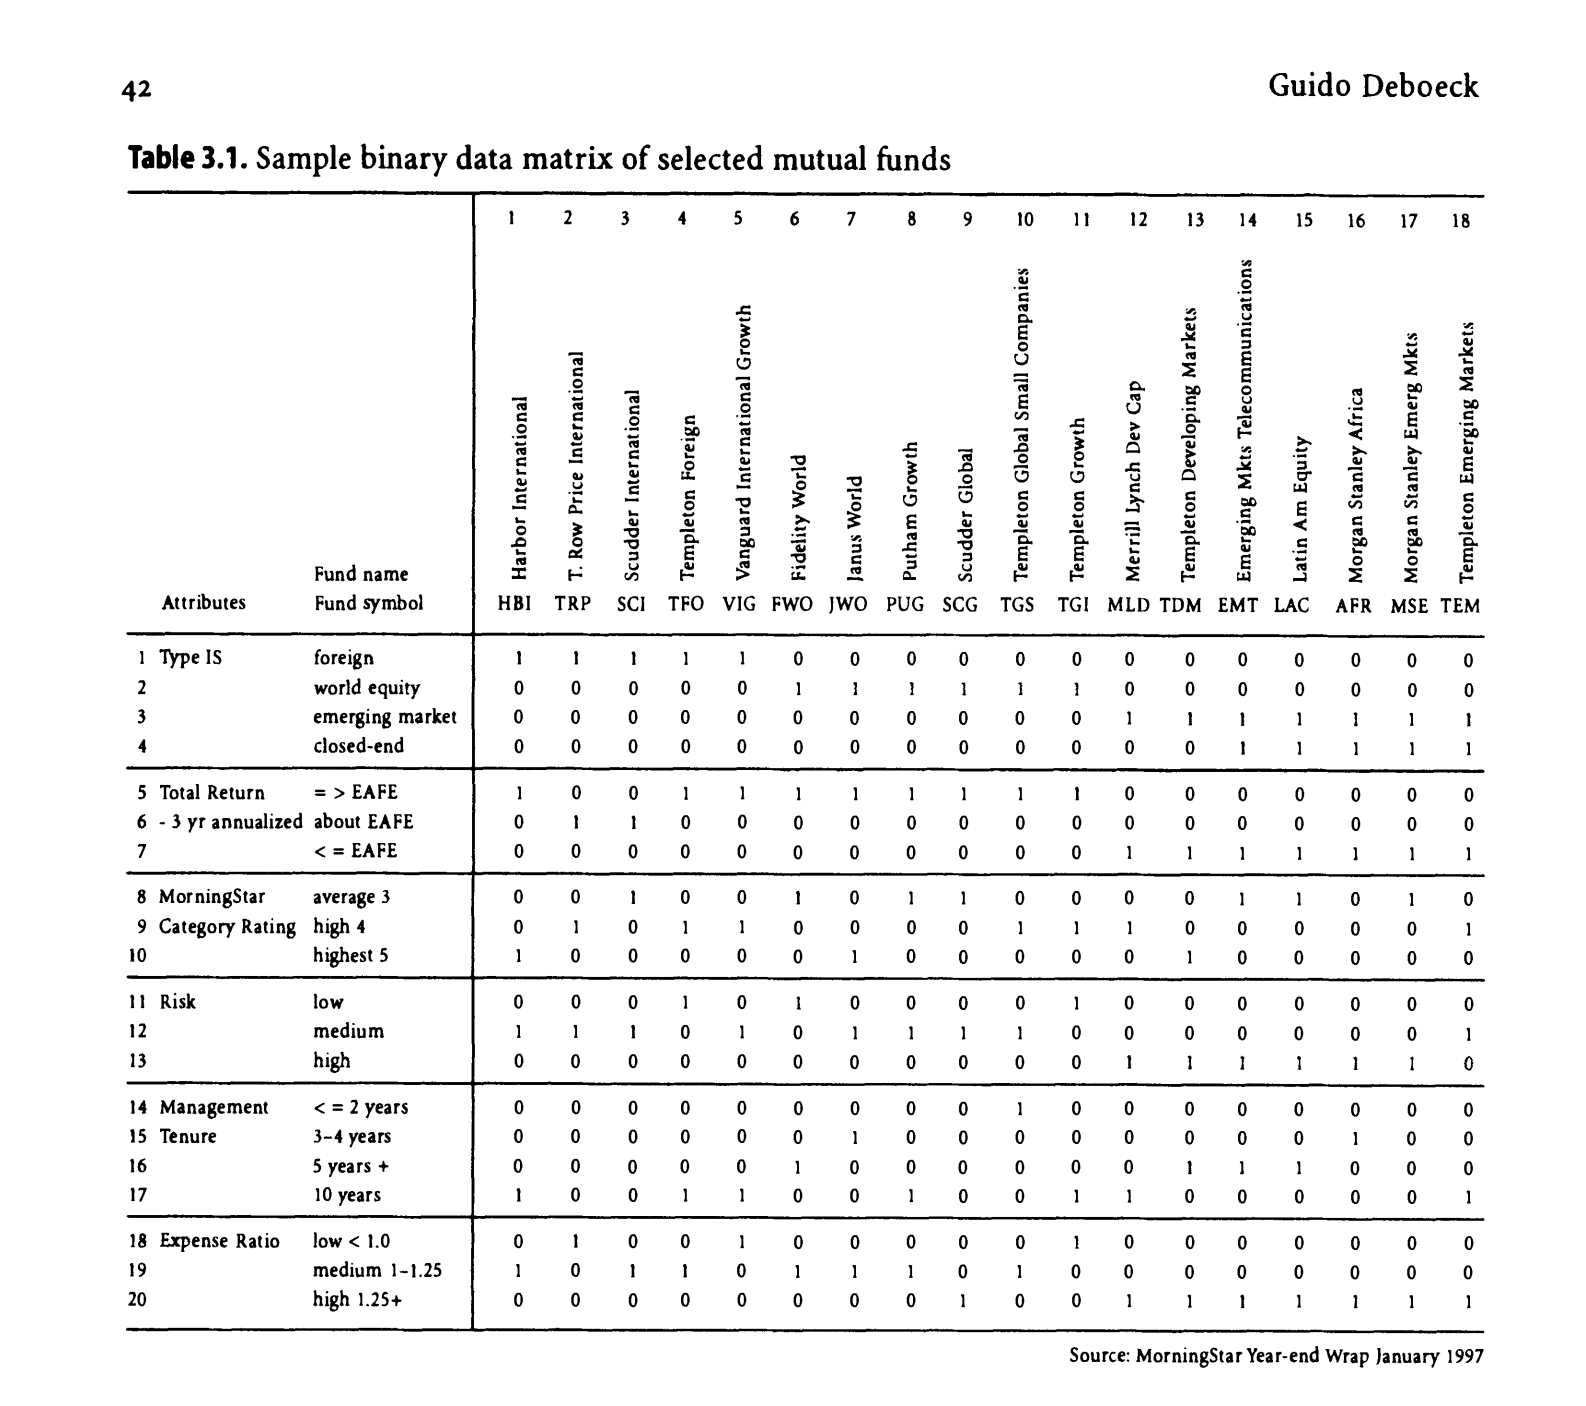
\includegraphics[width=0.5\textwidth]{Table3}
        \caption{Figura 3.1: \cite{Visual}}
      \end{wrapfigure}
      
      Con este trabajo se puede ver que los SOM simplifican clasificación de fondos;
      pueden usarse para el apoyo en la toma de decisiones; y para proporcionar
      clasificaciones que tienen más significado que las listas ordenadas basadas en múltiples
      criterios pues no necesitan hacer presuposiciones.

      Estos mapas se utiliza para buscar patrones entre mutual funds aparentemente similares. 
      La principal razon para usar SOM son:
      \begin{itemize}
        \item Es un método de minería de datos numérico en lugar de simbólico
        \item Es un método no paramétrico, lo que significa que no hay suposiciones a priori sobre
          como debe hacerse la distribución de los datos.
        \item Es un método que puede detectar estructuras o patrones inesperados mediante el aprendizaje
        sin supervisión.
      \end{itemize}

      \subsection{El dataset}

        Morningstar es una empresa privada fundada en 1984 para proporcionar a los inversores 
        información útil para tomar decisiones de inversión inteligentes e informadas. 
        
        Morningstar publica Morningstar Mutual Funds, una revista analítica exhaustiva sobre 
        mutual funds \Quote{Morningstar Investor}, este es un compendio mensual de 450 fondos abiertos
        y 50 fondos cerrados seleccionados de un universo de más de 6000 mutual funds. 
         
        Los 500 representan, según Morningstar, los fondos más exitosos en la industria de fondos 
        mutuos en la actualidad.

        Como pueden ver se trata de un dataset binario y que tiene 20 caracteristicas.


      \subsection{Arquitectura; fases de entrenamiento y clasificación}

        SOM de una matriz de datos de una muestra binaria, 
        se utilizo un tamaño de mapa de 10 por 1, donde la longitud inicial del
        entrenamiento fue de 1000 epochs.
        
        La tasa de aprendizaje inicial fue de 0.05 con un radio inicial de 5;
        
        La segunda fase del entrenamiento fue de 10,000 epochs, con una tasa de aprendizaje de 0.02
        y un radio de 1.

        Todos los pesos fueron inicializados con un número aleatorio al inicio y se uso la clásica distancia
        euleriana.

        \begin{figure}[h]
            \centering
            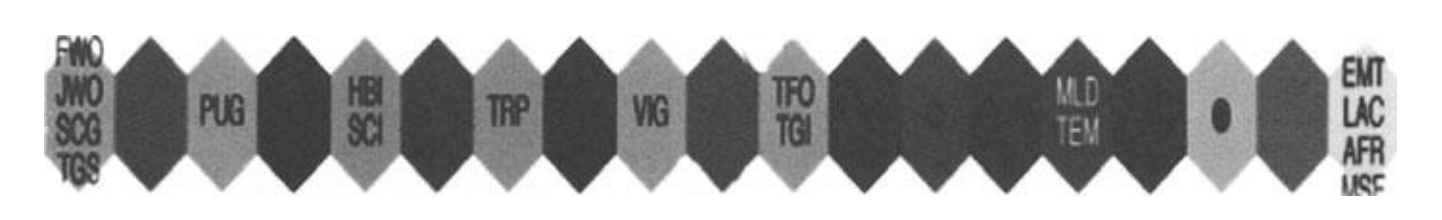
\includegraphics[width=0.85\textwidth]{Table1}
            \caption{Figura 3.3: \cite{Visual}}
        \end{figure}

        \begin{figure}[h]
            \centering
            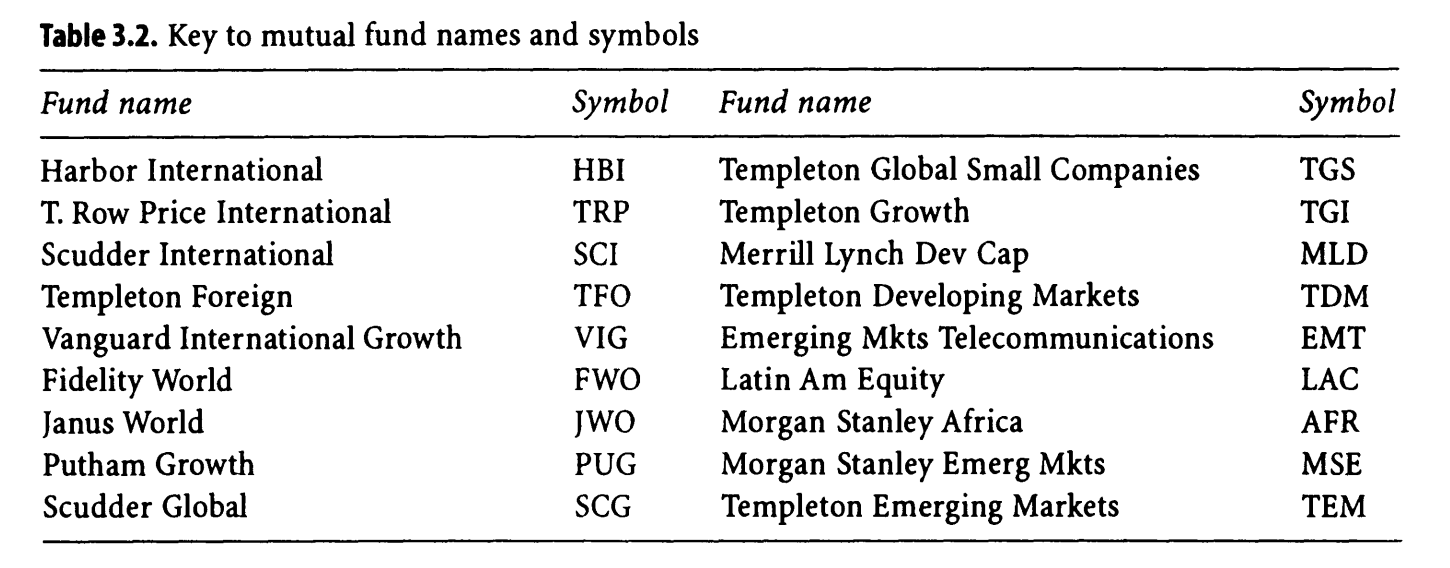
\includegraphics[width=0.85\textwidth]{Table2}
            \caption{Figura 3.2: \cite{Visual}}
        \end{figure}
        
      \subsection{Resultados}

        El primer ejemplo en el articulo es un SOM de 1 por 10 neuronas. 
        La figura 3.1 muestra que varios fondos de inversión se agrupan. 
        
        Por ejemplo, Fidelity World (FWO), Janus World OWO), Scudder Global (SCG) y Templeton 
        Global Small Companies (TGS) se agrupan en una neurona; 
        
        Las telecomunicaciones de mercados emergentes (EMT), la renta variable de América Latina (LAC), 
        Morgan Stanley África (AFR) y los mercados emergentes de Morgan Stanley (MSE) se 
        agrupan en otra neurona. 
        
        Hay otras tres neuronas que contienen dos mutual funds. 
        
        Dado que los vectores de entrada que son similares se agrupan en las mismas neuronas o 
        en las cercanas, las agrupaciones que se muestran en la Figura 3.1 indican la similitud 
        de los atributos de entrada entre los fondos que están en las mismas neuronas o en las cercanas.
        
        Para verificar esto, buscamos en la Tabla 3.1 el primer grupo listado y lo
        comparamos con el segundo grupo principal. 
        
        El primer grupo de fondos está más diversificado, mientras que el segundo grupo contiene
        fondos que están más enfocados en sectores específicos o regiones geográficas del mundo.
        EMT, por ejemplo, es un fondo que solo invierte en empresas de telecomunicaciones; ALC, AFR
        y MSE son fondos que se especializan en inversiones en América Latina, África 
        o mercados emergentes, respectivamente. 
        
        El sombreado gris de las neuronas en este mapa indica que esas neuronas con sombreado
        similar contienen mutual funds que están más cercanos entre sí, mientras que las 
        neuronas que están sombreadas de manera oscura crean brechas entre los grupos.


    \section{Ideas para usar mapas de Kohomen en la vida real}

        

      \subsection{Mi idea, arquitectura y demás}

      \begin{wrapfigure}{r}{0.4\textwidth}
        \centering
        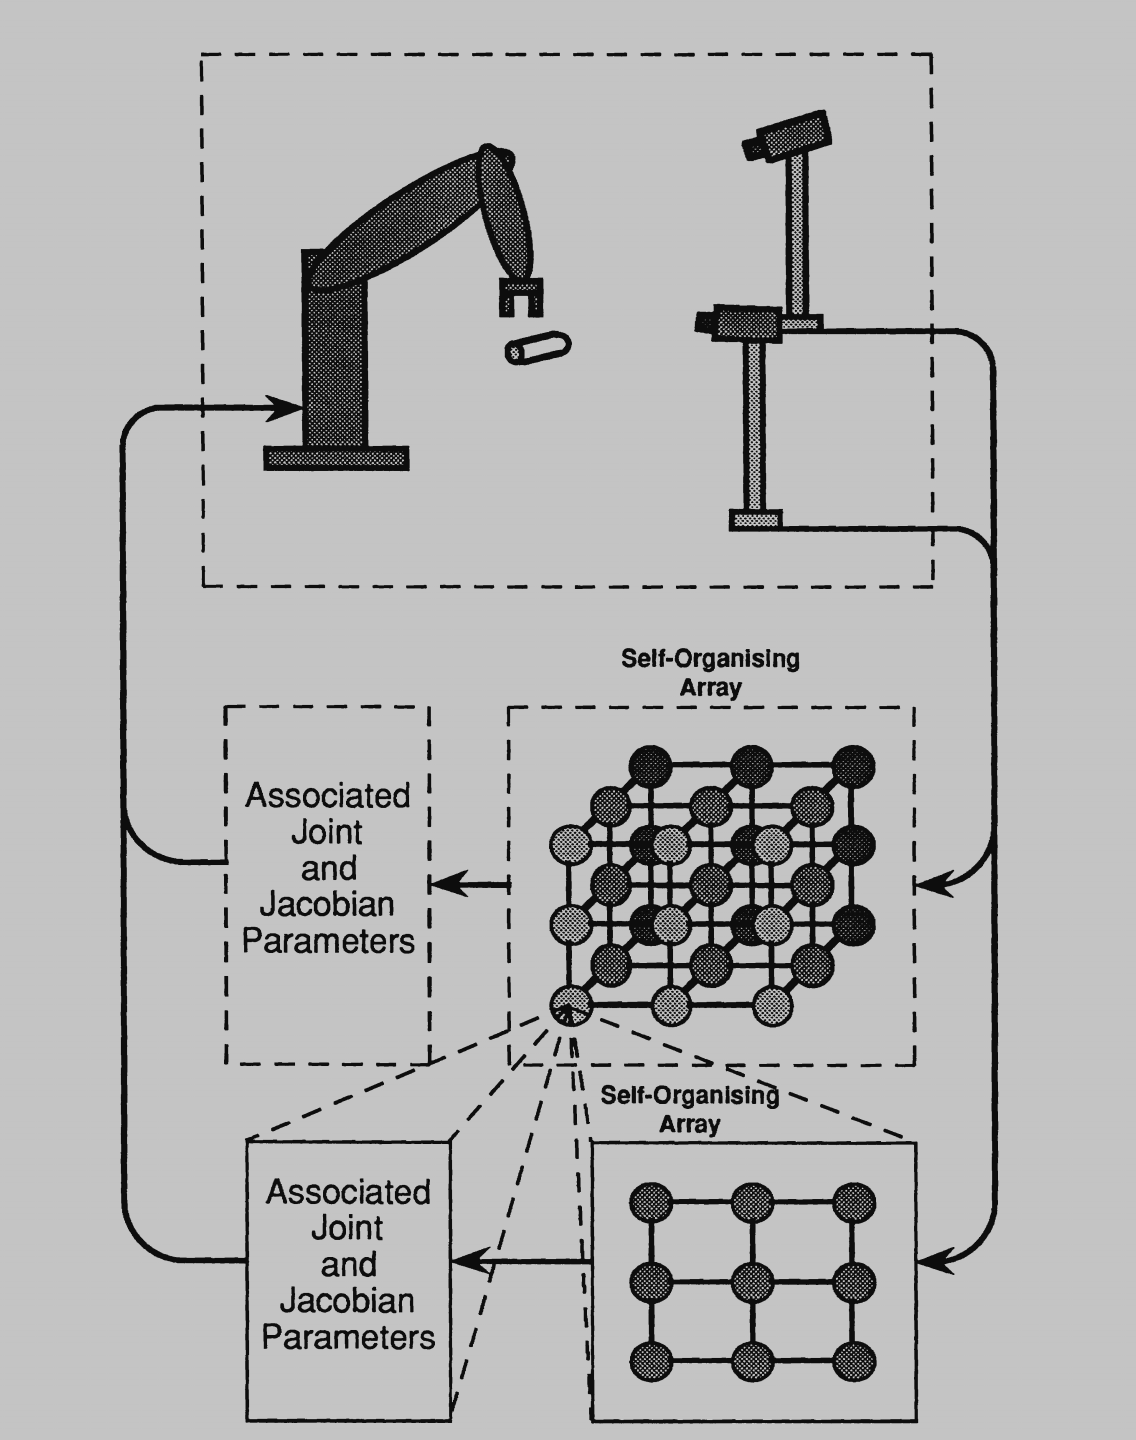
\includegraphics[width=0.4\textwidth]{Table5}
        \caption{ \cite{Robot}}
      \end{wrapfigure}


      Mi idea era desarrollar un mapa que le permitiera a un robot aprender como
      estaban relacionados los movimientos de los que era capaz, por ejemplo
      supongamos que tenemos un robot con 5 o 6 grados de libertad, en ese caso
      podemos usar un mapa autorganizado para poder visualizar de manera sencilla
      que patrones existen dentro de los movimientos que realiza el robot, investigando un poco
      mas me encontre con que ya existe estas ideas, asi que ahora no puedo decir que es mi dia porque
      me vi influido por otros, en especial por una
      red desarrollada por Saxon y Mukerjee que aprende el mapa de movimiento de un 
      brazo robotico de dos grados de libertad utilizando un mapa de características 
      autoorganizadas. 
      
      Este mapa se puede utilizar para planificar una ruta con el fin de evitar obstáculos.
      El sistema utiliza un mapa de características en 2D del como las  propuestas por Kohonen.

      La idea seria tener un mapa que recibe cuatro entradas: dos que representan la posición en el espacio cartesiano
      del efector final y dos que representan la posición del espacio articular (angulos) del efector final.

      El sistema se entrena moviendo el brazo a un punto aleatorio en el espacio articular, y
      con esto registrando la posición cartesiana del efector final y luego alimentando la información 
      cartesiana y articular a la red.
      
      Después de muchos miles, y miles de estos movimientos, el sistema debería
      aprender un mapeo topológico del espacio de entrada. 
      
      En esencia, cada neurona representa un punto en el espacio cartesiano y 
      un punto en el espacio articular.

      Una vez que se hubiera aprendido el mapa de movimiento, entonces tenemos la base 
      para un medio bastante elegante de planificar trayectorias alrededor de obstáculos 
      como lo describen Saxon y Mukerjee. 
      
      La idea básica es que cada neurona en la red 2-D corresponde tanto a un 
      espacio articular como a una posición de espacio cartesiano. 
      
      Por lo tanto realizar la planificación de la trayectoria utilizando esta red 
      permite la incorporación de información tanto de espacios articulares como cartesianos, 
      mientras que solo requiere que se busque una matriz 2D de posibles caminos. (lo cual
      puede potencialmente mejorar en gran medida la complejidad algoritmia de tiempo 
      en la busqueda).
      
      Se pueden incorporar obstáculos desactivando las entradas del espacio articular a la red, 
      aplicando la posición del espacio cartesiano de los objetos a la red y
      luego desactivando las neuronas que produjeron respuestas máximas. 
      
      Luego, se puede determinar una posible trayectoria que evite estos obstáculos
      eligiendo un camino a través de la matriz neural 2-D que comienza en la neurona
      que representa más parecido a la posición actual del espacio articular del brazo, 
      evitando las neuronas que se han desactivado y terminando en el punto que representa la posicion
      más cercana a la posición deseada del efector final (en espacio articular o cartesiano).

      Dadas las caracteristicas de este problema podriamos sin ningun problema empezar en pesos aleatorios
      y usar la clasica distancia euleriana pues justo estamos hablando de problemas en lo que estamos
      mapeando al mundo real, por lo que resulta una forma de medir distancias bastante prometedora
      a priori.

    \subsection{¿Porque es diferente a las demas redes?}

      Esta red es claramente diferente a todas las demas que hemos visto a lo largo del curso
      primeramente porque se trata de aprendizaje no supervisado, por lo que a finalidad es 
      tomar un monton de datos y usar estos mapa para poder extraer caracteristicas de la informacion.

      En otras palabras: Los Mapas autorganizados de Kohonen son un
      tipo de red neuronal utilizado en problemas de reconocimiento de patrones.

      Es especialmente capaz de agrupar y visualizar datos complejos de altas dimensiones y
      puede aplicarse potencialmente para resolver muchos problemas complejos del mundo real.

      Si bien podemos argumentar que por ejemplo las redes convolucionales tambien son
      redes en las que ellas mismas aprenden los patrones necesarios para reconocer clases,
      esto es diferente y es justo en lo que acabo de decir, pues en el caso de las convolucionales
      ya tenemos unas clases dadas mientras que con estas podemos generar clases automaticamente.

      Ahora el problema que acabamos de ver seria bastante dificil que hacer usando una red
      neuronal como las anteriores, de mismo modo que la idea que acabo de contar, pues por ejemplo
      para el brazo robotico tendriamos que darle a una red neuronal la relación (y encontrar
      una forma de cuantificar la relación) que existe entre las dimensiones cartesianas y las 
      de articulaciones, pero en que en mi ejemplo justo lo que no tenemos son dichas relaciones
      y usamos los mapas autorganizados para encontrarlas.

    \subsection{Desafios}

      Uno de los principales problemas a los que me podria enfrentar es que la gente me dijera
      que para sistemas bien definidos, como este caso,  a menudo será mucho más rápido calcular
      una respuesta exacta en lugar de utilizar un mapa autorganizados para obtener una 
      solución aproximada. 
      
      Esto es particularmente cierto cuando se emplea un procesador secuencial.

      Tambien habria que ver que al ser aprendizaje no supervisado necesitamos grandes cantidades de 
      datos, mismos que quiza podrian contener una gran cantidad de errores (sobretodo con el uso de
      sensores) y sin conocer la relacion per ser nos seria bastante dificil para nosotros saber si 
      la informacion que le estamos ingresando a la red es 100\% correcta.

      Tambien elegir correctamente el espacio de salida y el radio de \Quote{vecindad}.

  \section{¿Porqué la tasa de aprendizaje baja?}

    La selección de un factor de ganancia adecuado (learning rate), parece ser un compromiso entre la
    tasa de aprendizaje y la precisión del aprendizaje. 
    
    Si se elige un factor de alta ganancia, el aprendizaje continuará rápidamente, 
    pero la red cambiará constantemente con cada nuevo patrón de entrada y, por lo tanto, 
    es posible que no se clasifique de manera uniforme todo el espacio de entrada. 
    
    Por otro lado, si eligimos un factor de baja ganancia, entonces el 
    aprendizaje será muy lento pero eventualmente debería alcanzar un resultado muy preciso. 
    Por lo tanto, el factor de ganancia generalmente se elige para ser inicialmente bastante
    grande (para asegurar un aprendizaje inicial rápido) y luego se reduce para aumentar la
    precisión del resultado final.

    Kohonen ha demostrado que una red unidimensional de neuronas con una sola entrada formará 
    un mapeo ordenado siempre que alfa sea menor que uno. 
    Sin embargo, no está claro que esta prueba se escalara para los casos en que la entrada o 
    la red fueran de mayor dimensionalidad. 
    
    En particular, es poco probable que se aplique para el caso donde la entrada tenía una 
    dimensión mucho más alta que la red. 

    La decisión sobre qué tamaño de vecindario se debe usar también parece determinarse de 
    una manera un tanto ad hoc.

  \section{Ideas biológicas}

    Parece claro que, al menos que los mamíferos se refieren, el 
    cerebro contiene un registro de la información sensorial previa. 
    Además, dado que el número de entradas posibles supera mucho el número de 
    neuronas en el cerebro parece claro que se produce una forma de compresión (o abstracción). 
    
    El mecanismo por el cual el cerebro almacena estas representaciones comprimidas no está 
    bien entendida, sin embargo, se hace las hipótesis que se registran en grandes hojas
    de neuronas en dos dimensiones y organizadas topologicamente". (me costo mucho entender y traducir
    este termino de la literatura, originalmente se llaman:  "2-D
    metrically and topologically organized" sheets of neural cells)
    
    En otras palabras el cerebro forma un mapeo entre el espacio de entrada 
    multidimensional y el de dos dimensiones de las neuronas.
    
    Hay unas evidencias para esta idea. Se han encontrado encontrado en la
    parte del cerebro donde se procesa el sonido en los mamíferos las neuronas 
    responden selectivamente a los sonidos de diferentes frecuencias. 
    
    De manera que la ubicación de una neurona parece estar directamente relacionada con la 
    frecuencia de del sonido de entrada.

    Se han encontrado otras representaciones topográficas en la zona de procesamiento visual,
    sensorial y motor del cerebro.

    Las redes de Kohonen son un intento, mas bien modesto de modelar el funcionamento del
    cerebro en esta regiones.

  \section{Desventajas de este tipo de red}

    Otra desventaja ademas de toda las que ya hemos dicho antes es que que el comportamiento 
    de estas redes no está bien definido matemáticamente.
    
    Esto significa que la selección de parámetros de red (como factores de ganancia y tamaños de 
    vecindad) debe realizarse de una manera un tanto ad hoc. 
    
    En particular existe la preocupación de una falta de garantía de que una red, 
    que tiene permitido adaptarse en el mundo real, siempre mantendrá un mapeo ordenado consistente.

  \section{Cosas curiosas}

      Resulta que investigando todo esto encontre con que hay alguien (Eklavya Sarkar) que
      como tesis hizo unas visualizaciones de estos mapas, anexo la tesis y varios screenshots 
      del resultado.

      Porque resulta que el codigo que uso puede ser visto facilmente montando un servidor
      basado en sus codigos en github. \cite{Tesis}

      \begin{figure}[h!]
        \centering
        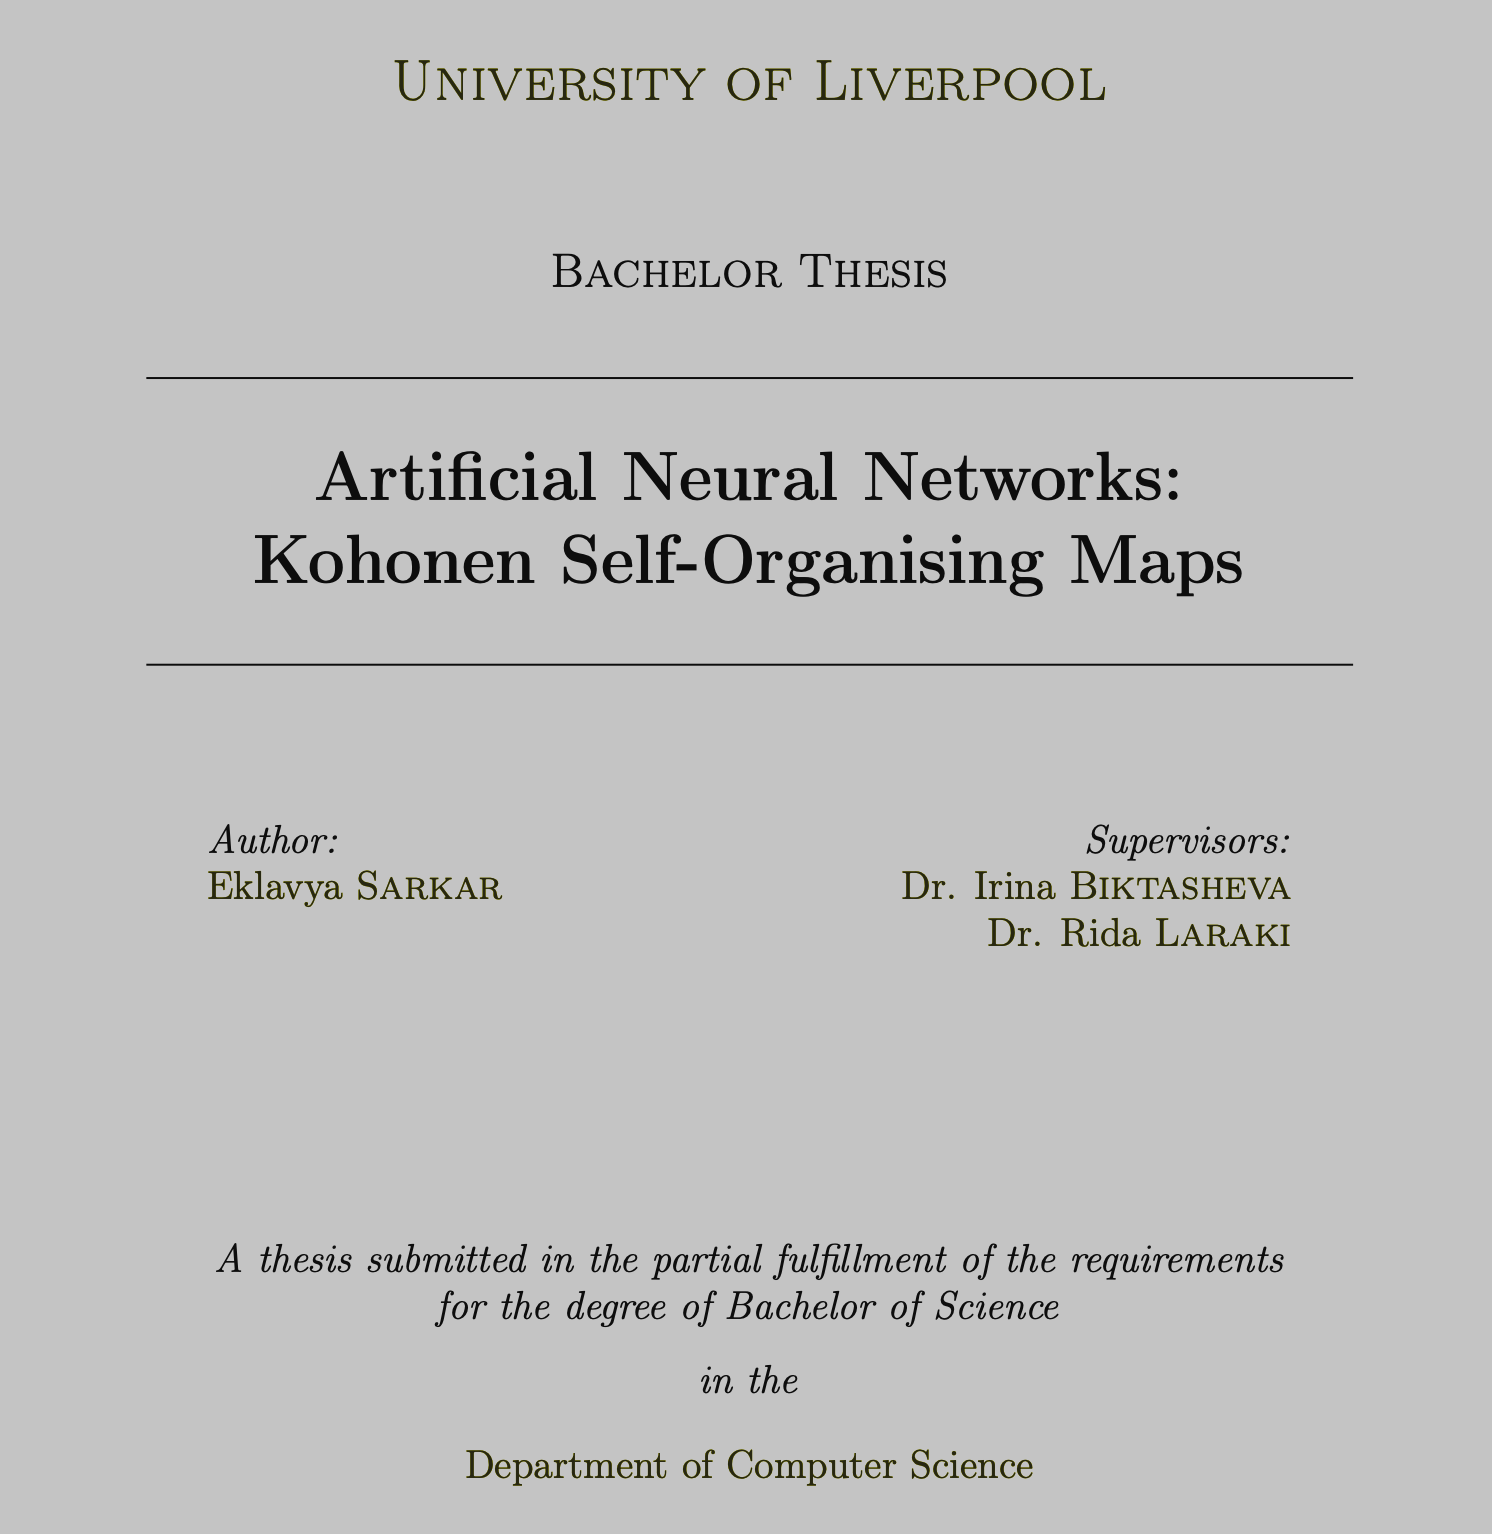
\includegraphics[width=\textwidth]{Tesis1}
      \end{figure}

      \begin{figure}[h!]
        \centering
        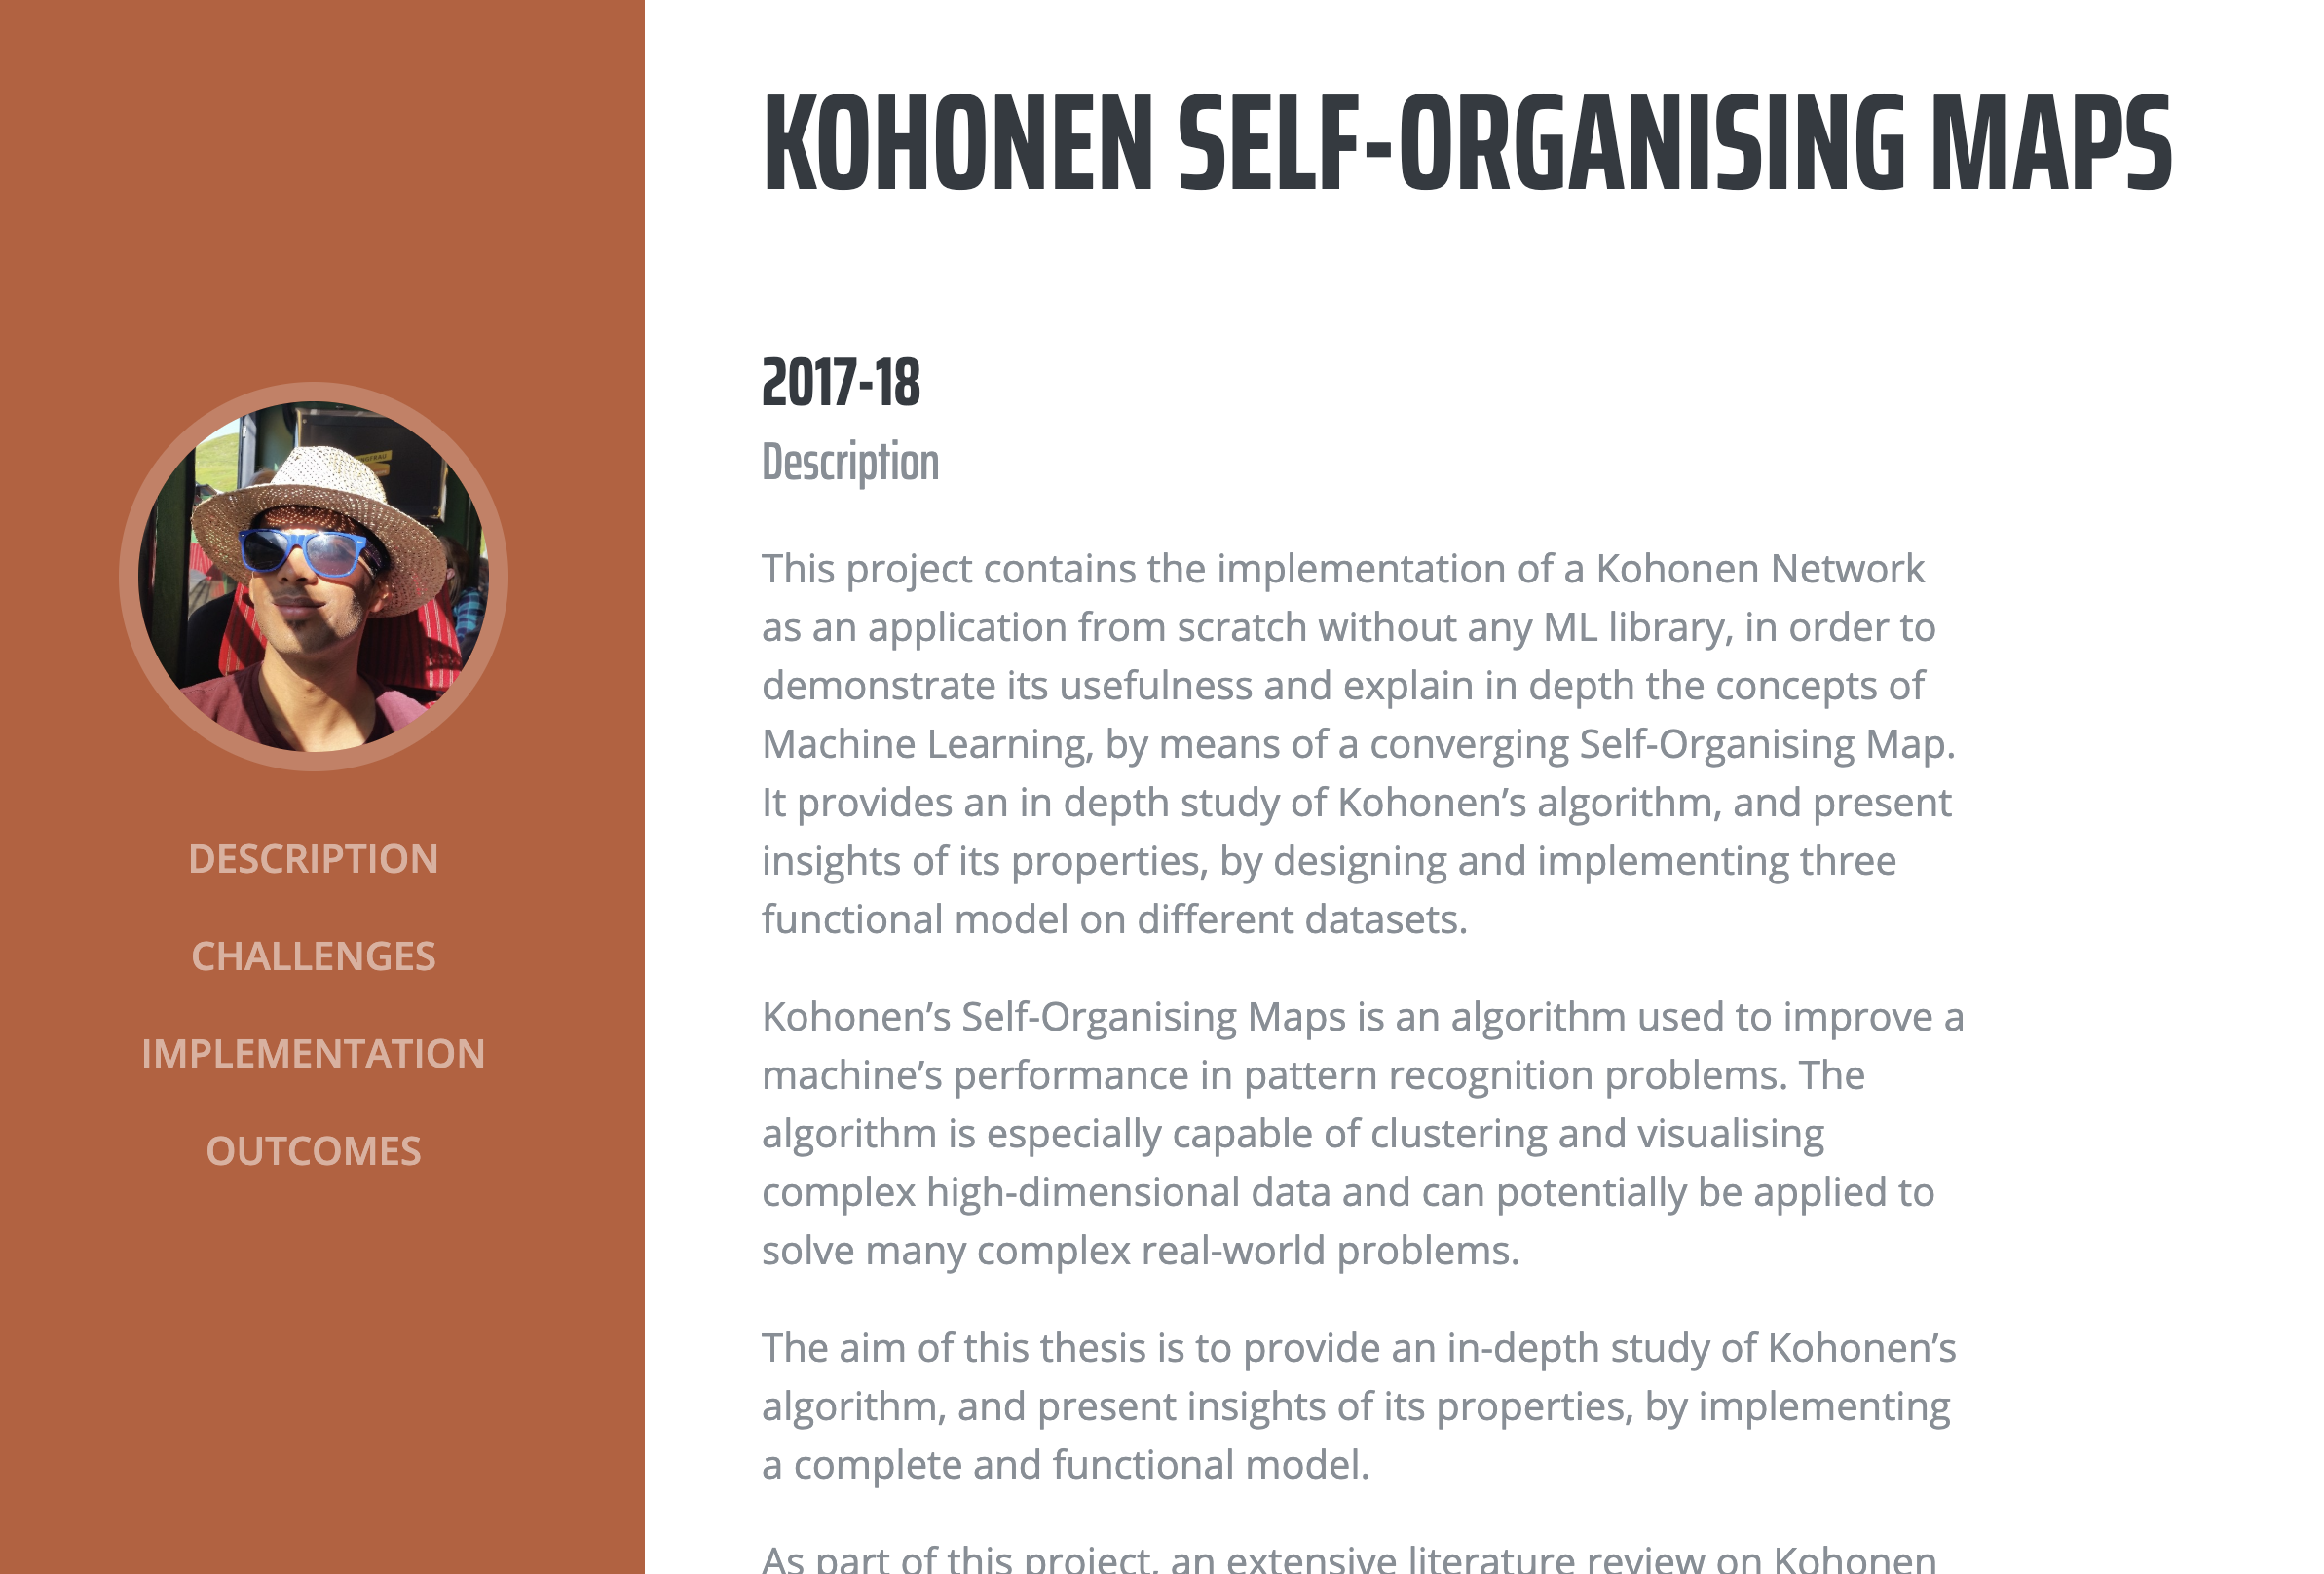
\includegraphics[width=\textwidth]{Tesis2}
      \end{figure}

      \begin{figure}[h!]
        \centering
        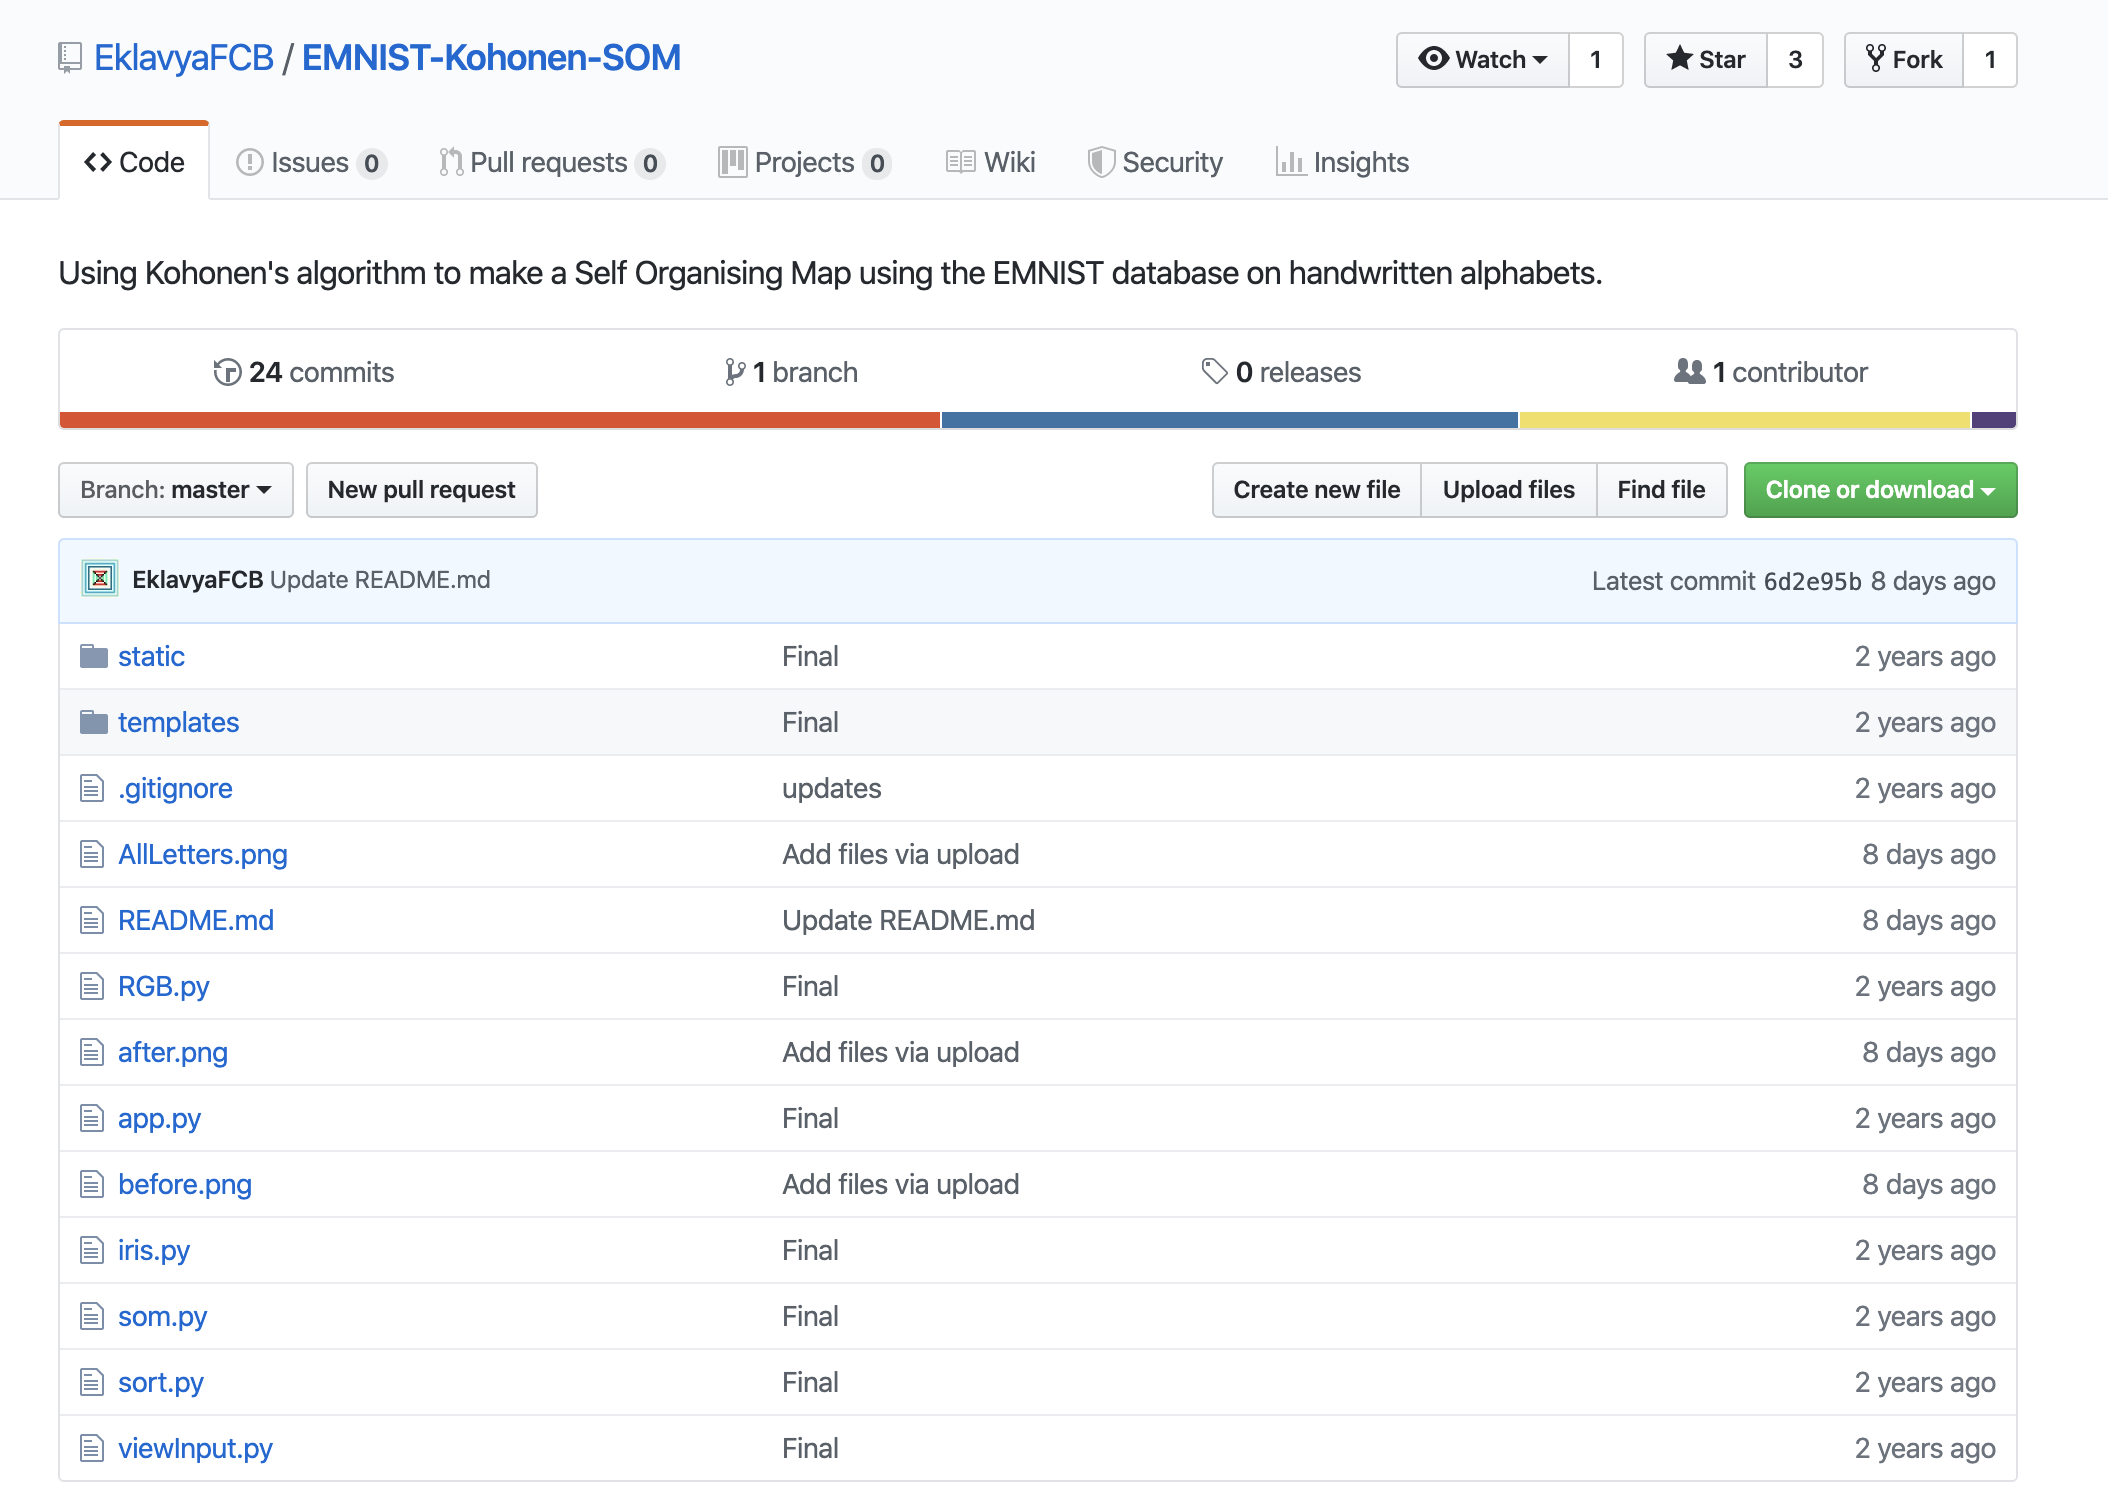
\includegraphics[width=\textwidth]{Tesis3}
      \end{figure}

      \begin{figure}[h!]
        \centering
        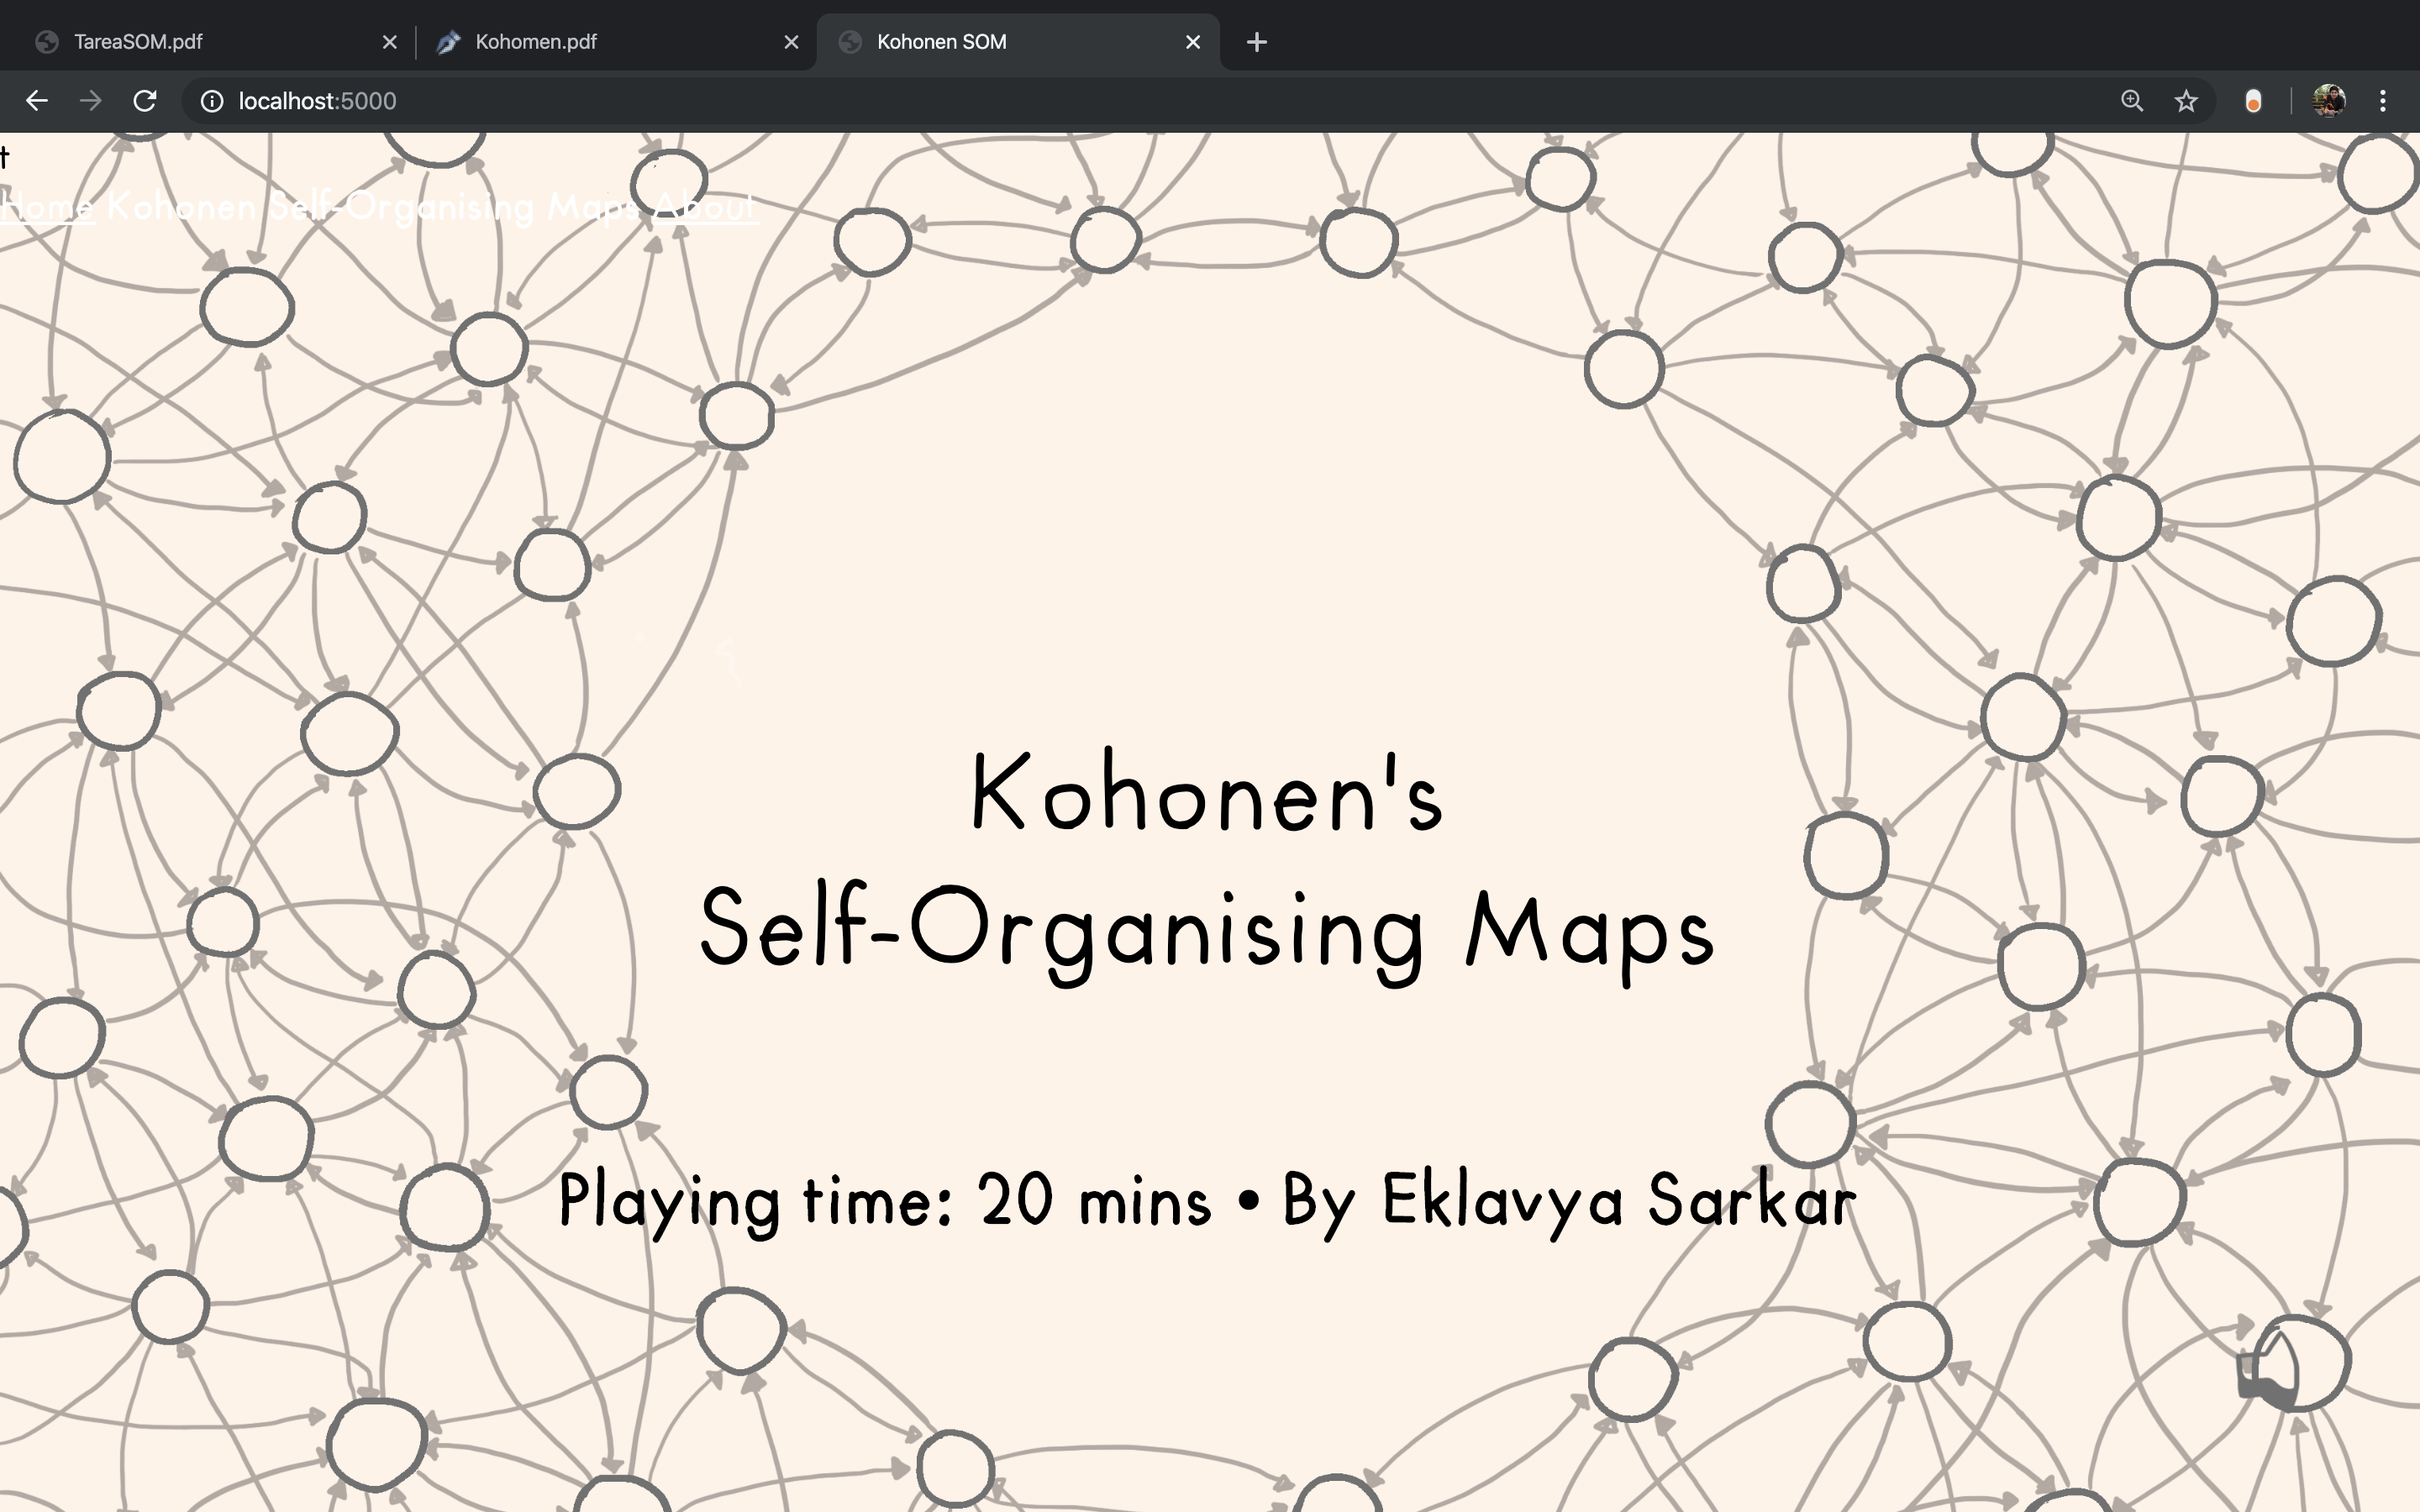
\includegraphics[width=\textwidth]{Tesis4}
      \end{figure}

      \begin{figure}[h!]
        \centering
        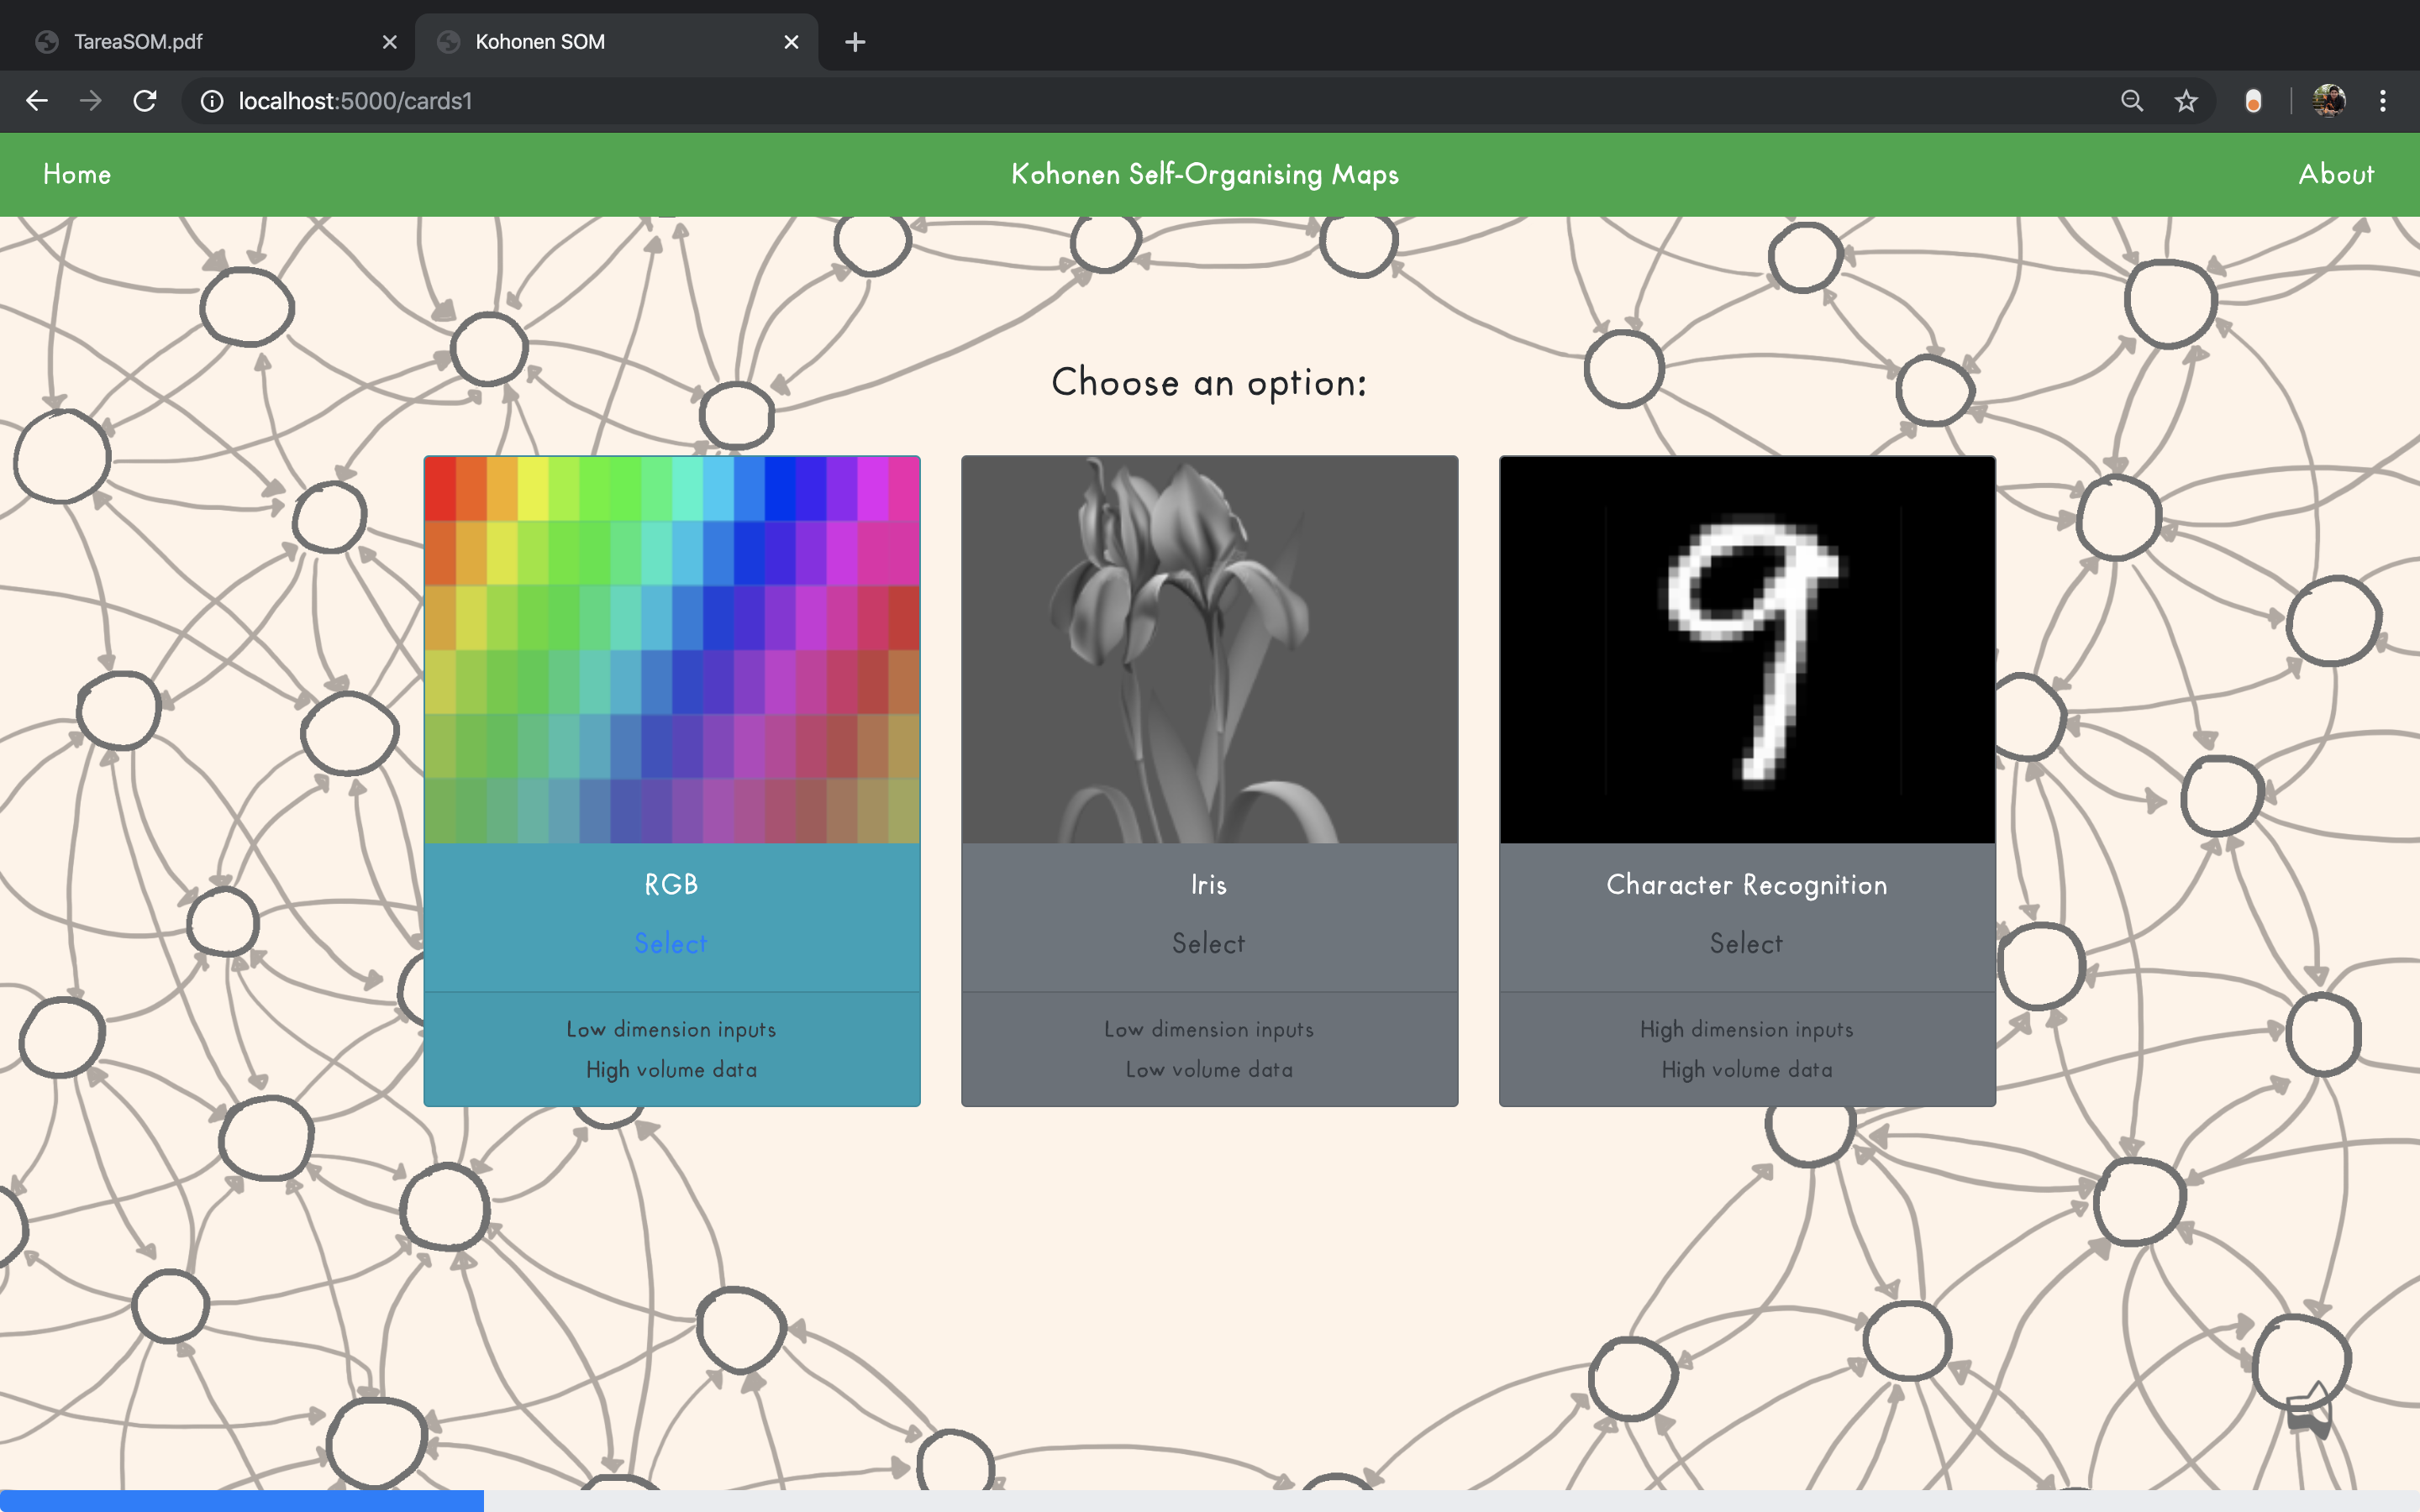
\includegraphics[width=\textwidth]{Tesis5}
      \end{figure}

      \begin{figure}[h!]
        \centering
        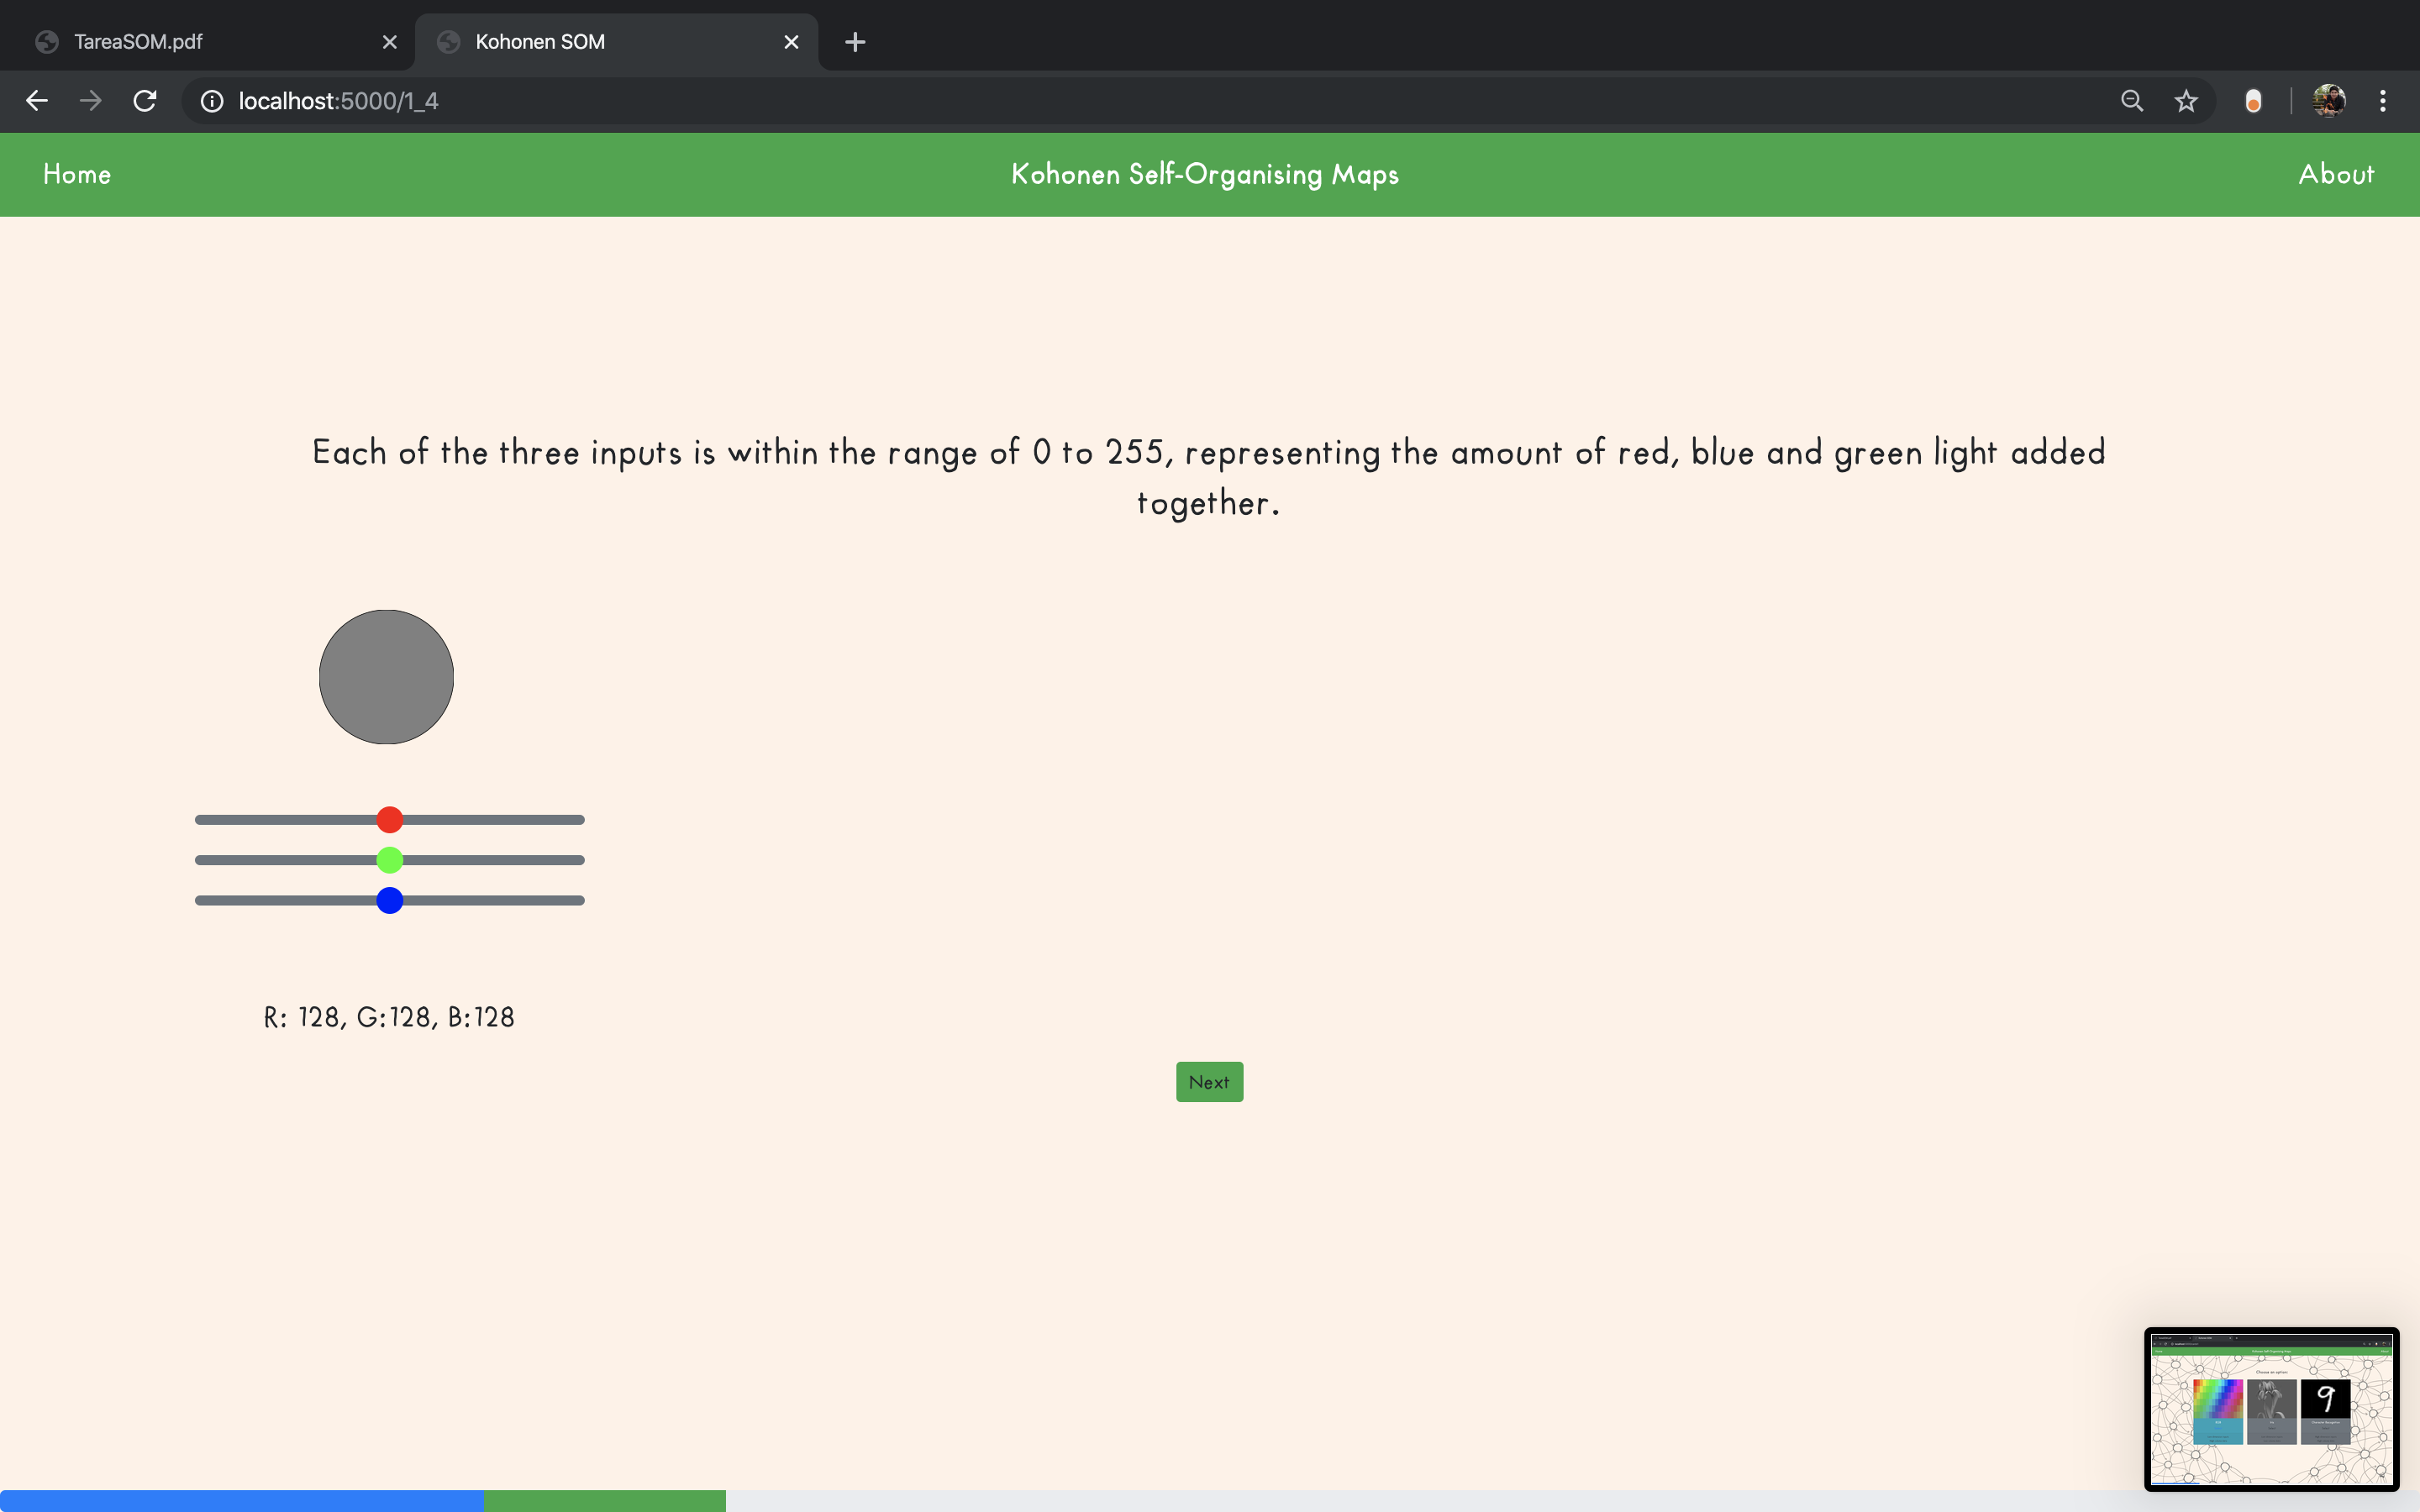
\includegraphics[width=\textwidth]{Tesis6}
      \end{figure}

      \begin{figure}[h!]
        \centering
        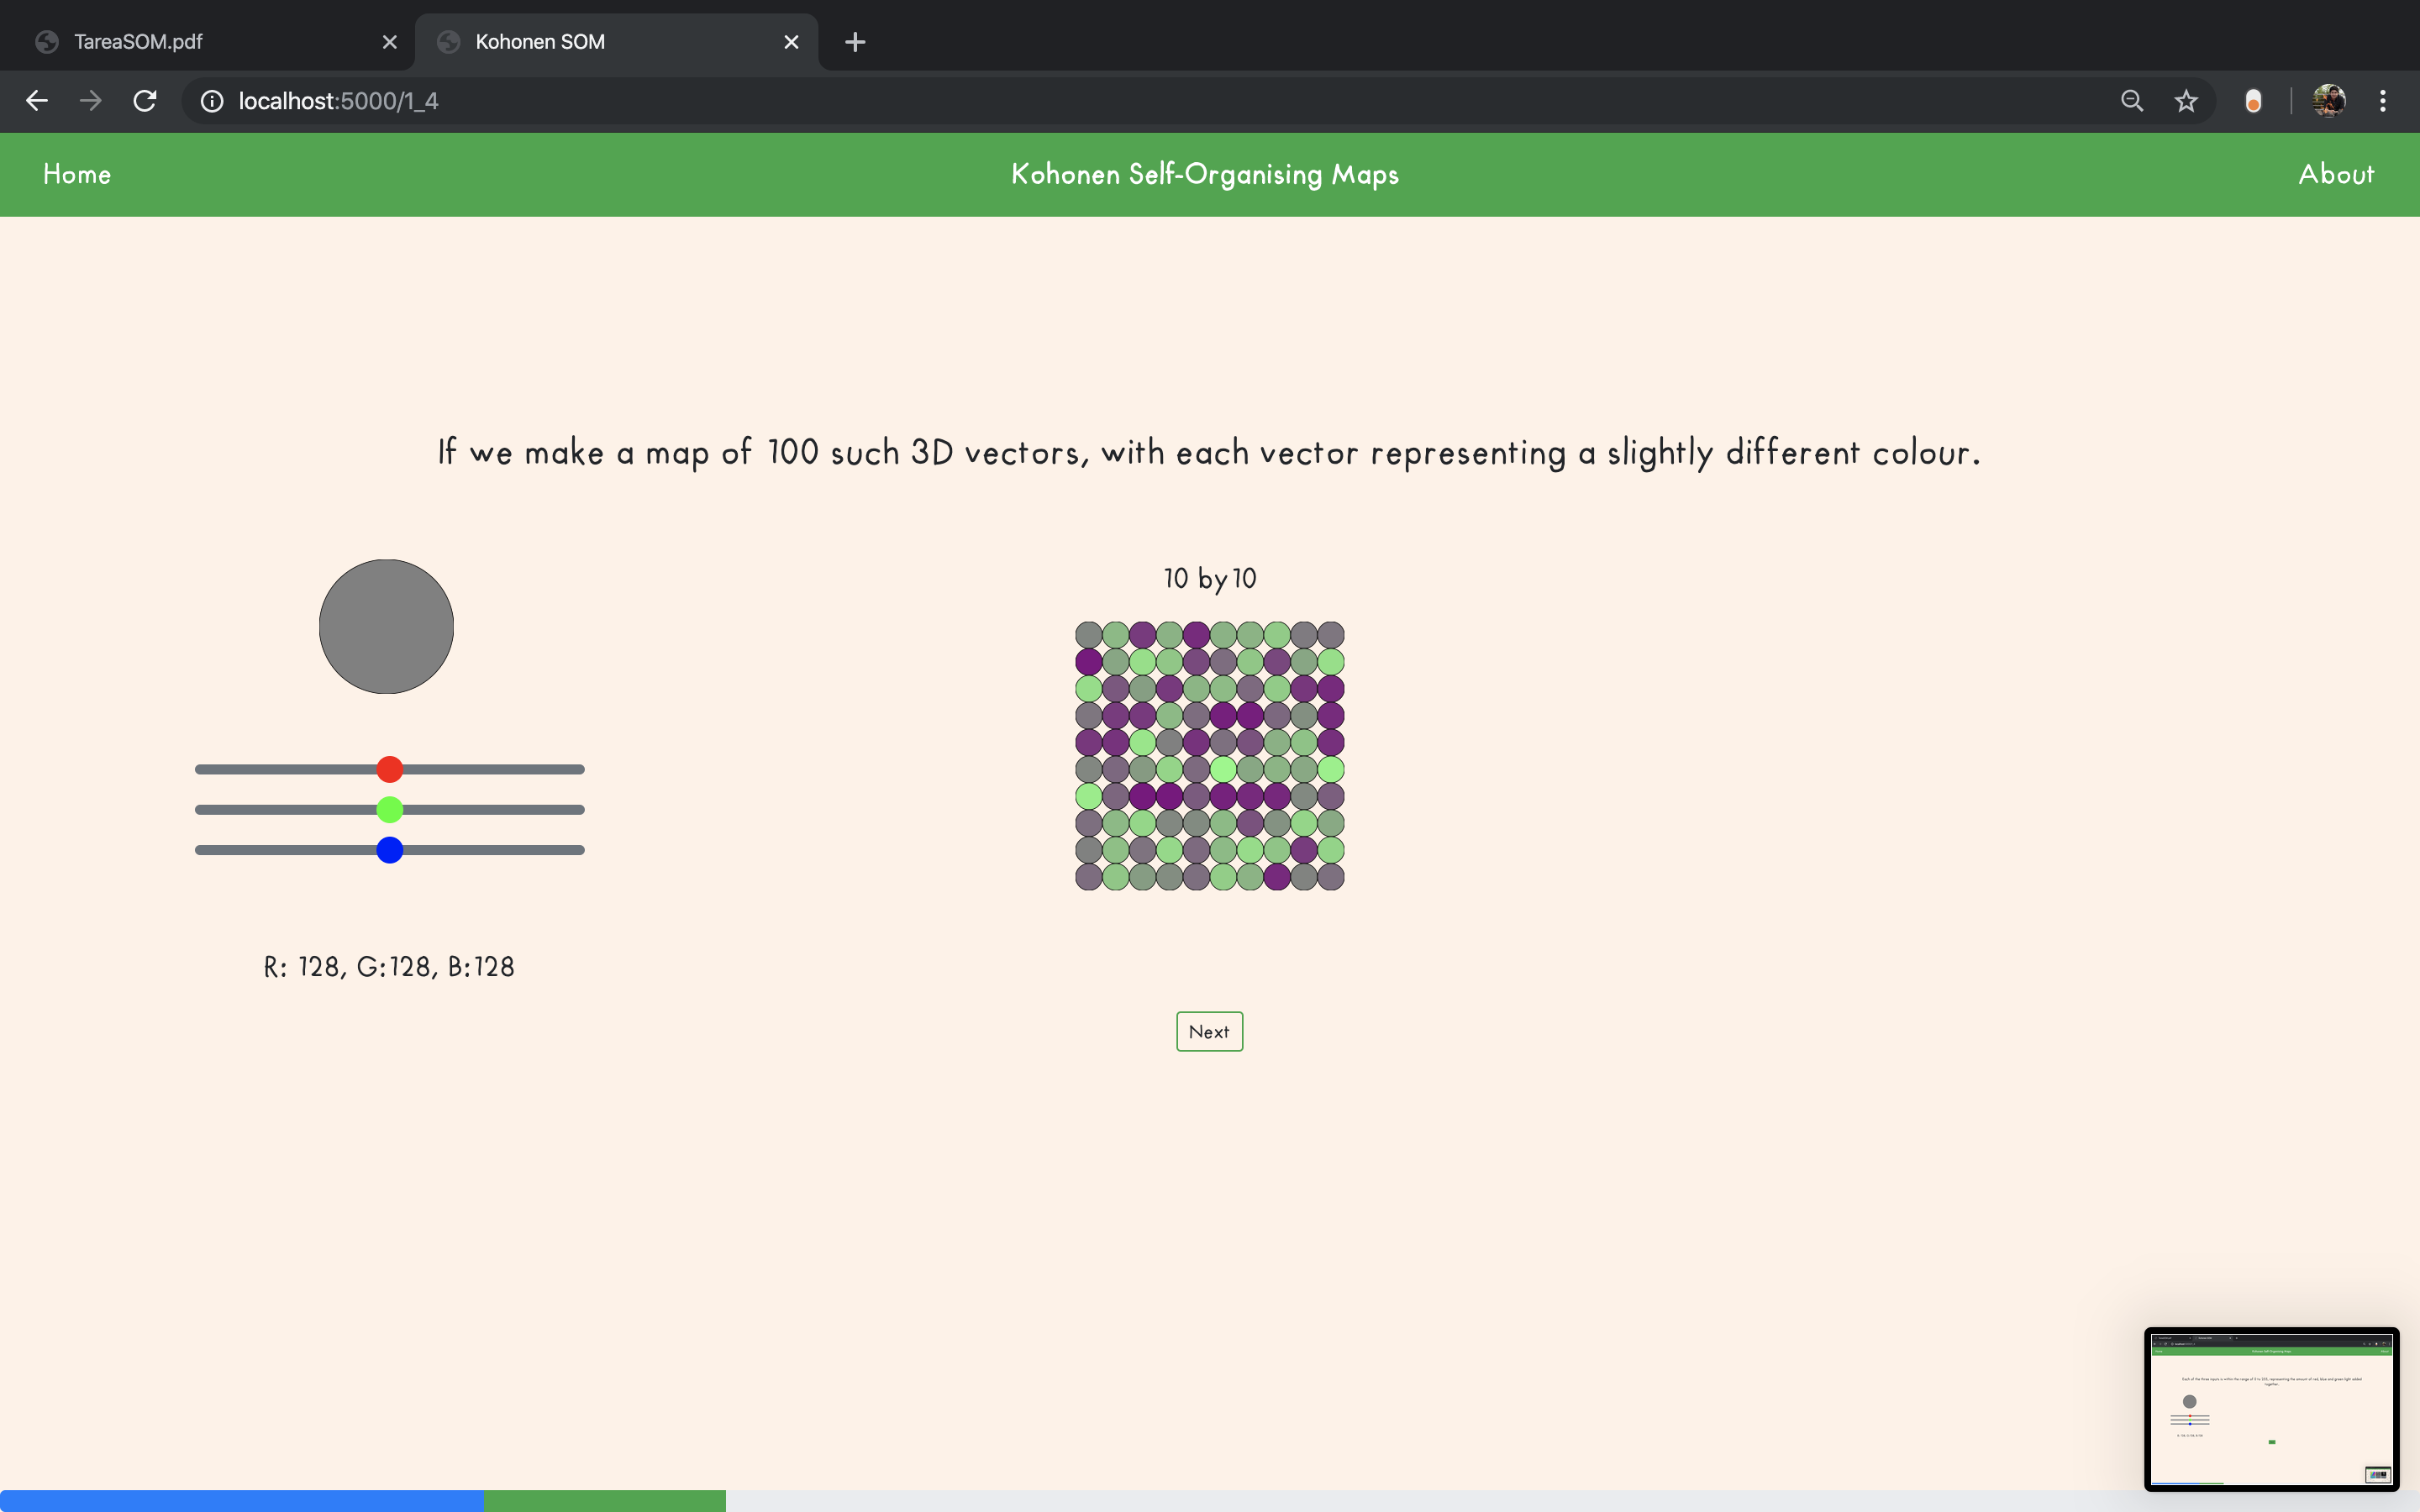
\includegraphics[width=\textwidth]{Tesis7}
      \end{figure}

      \begin{figure}[h!]
        \centering
        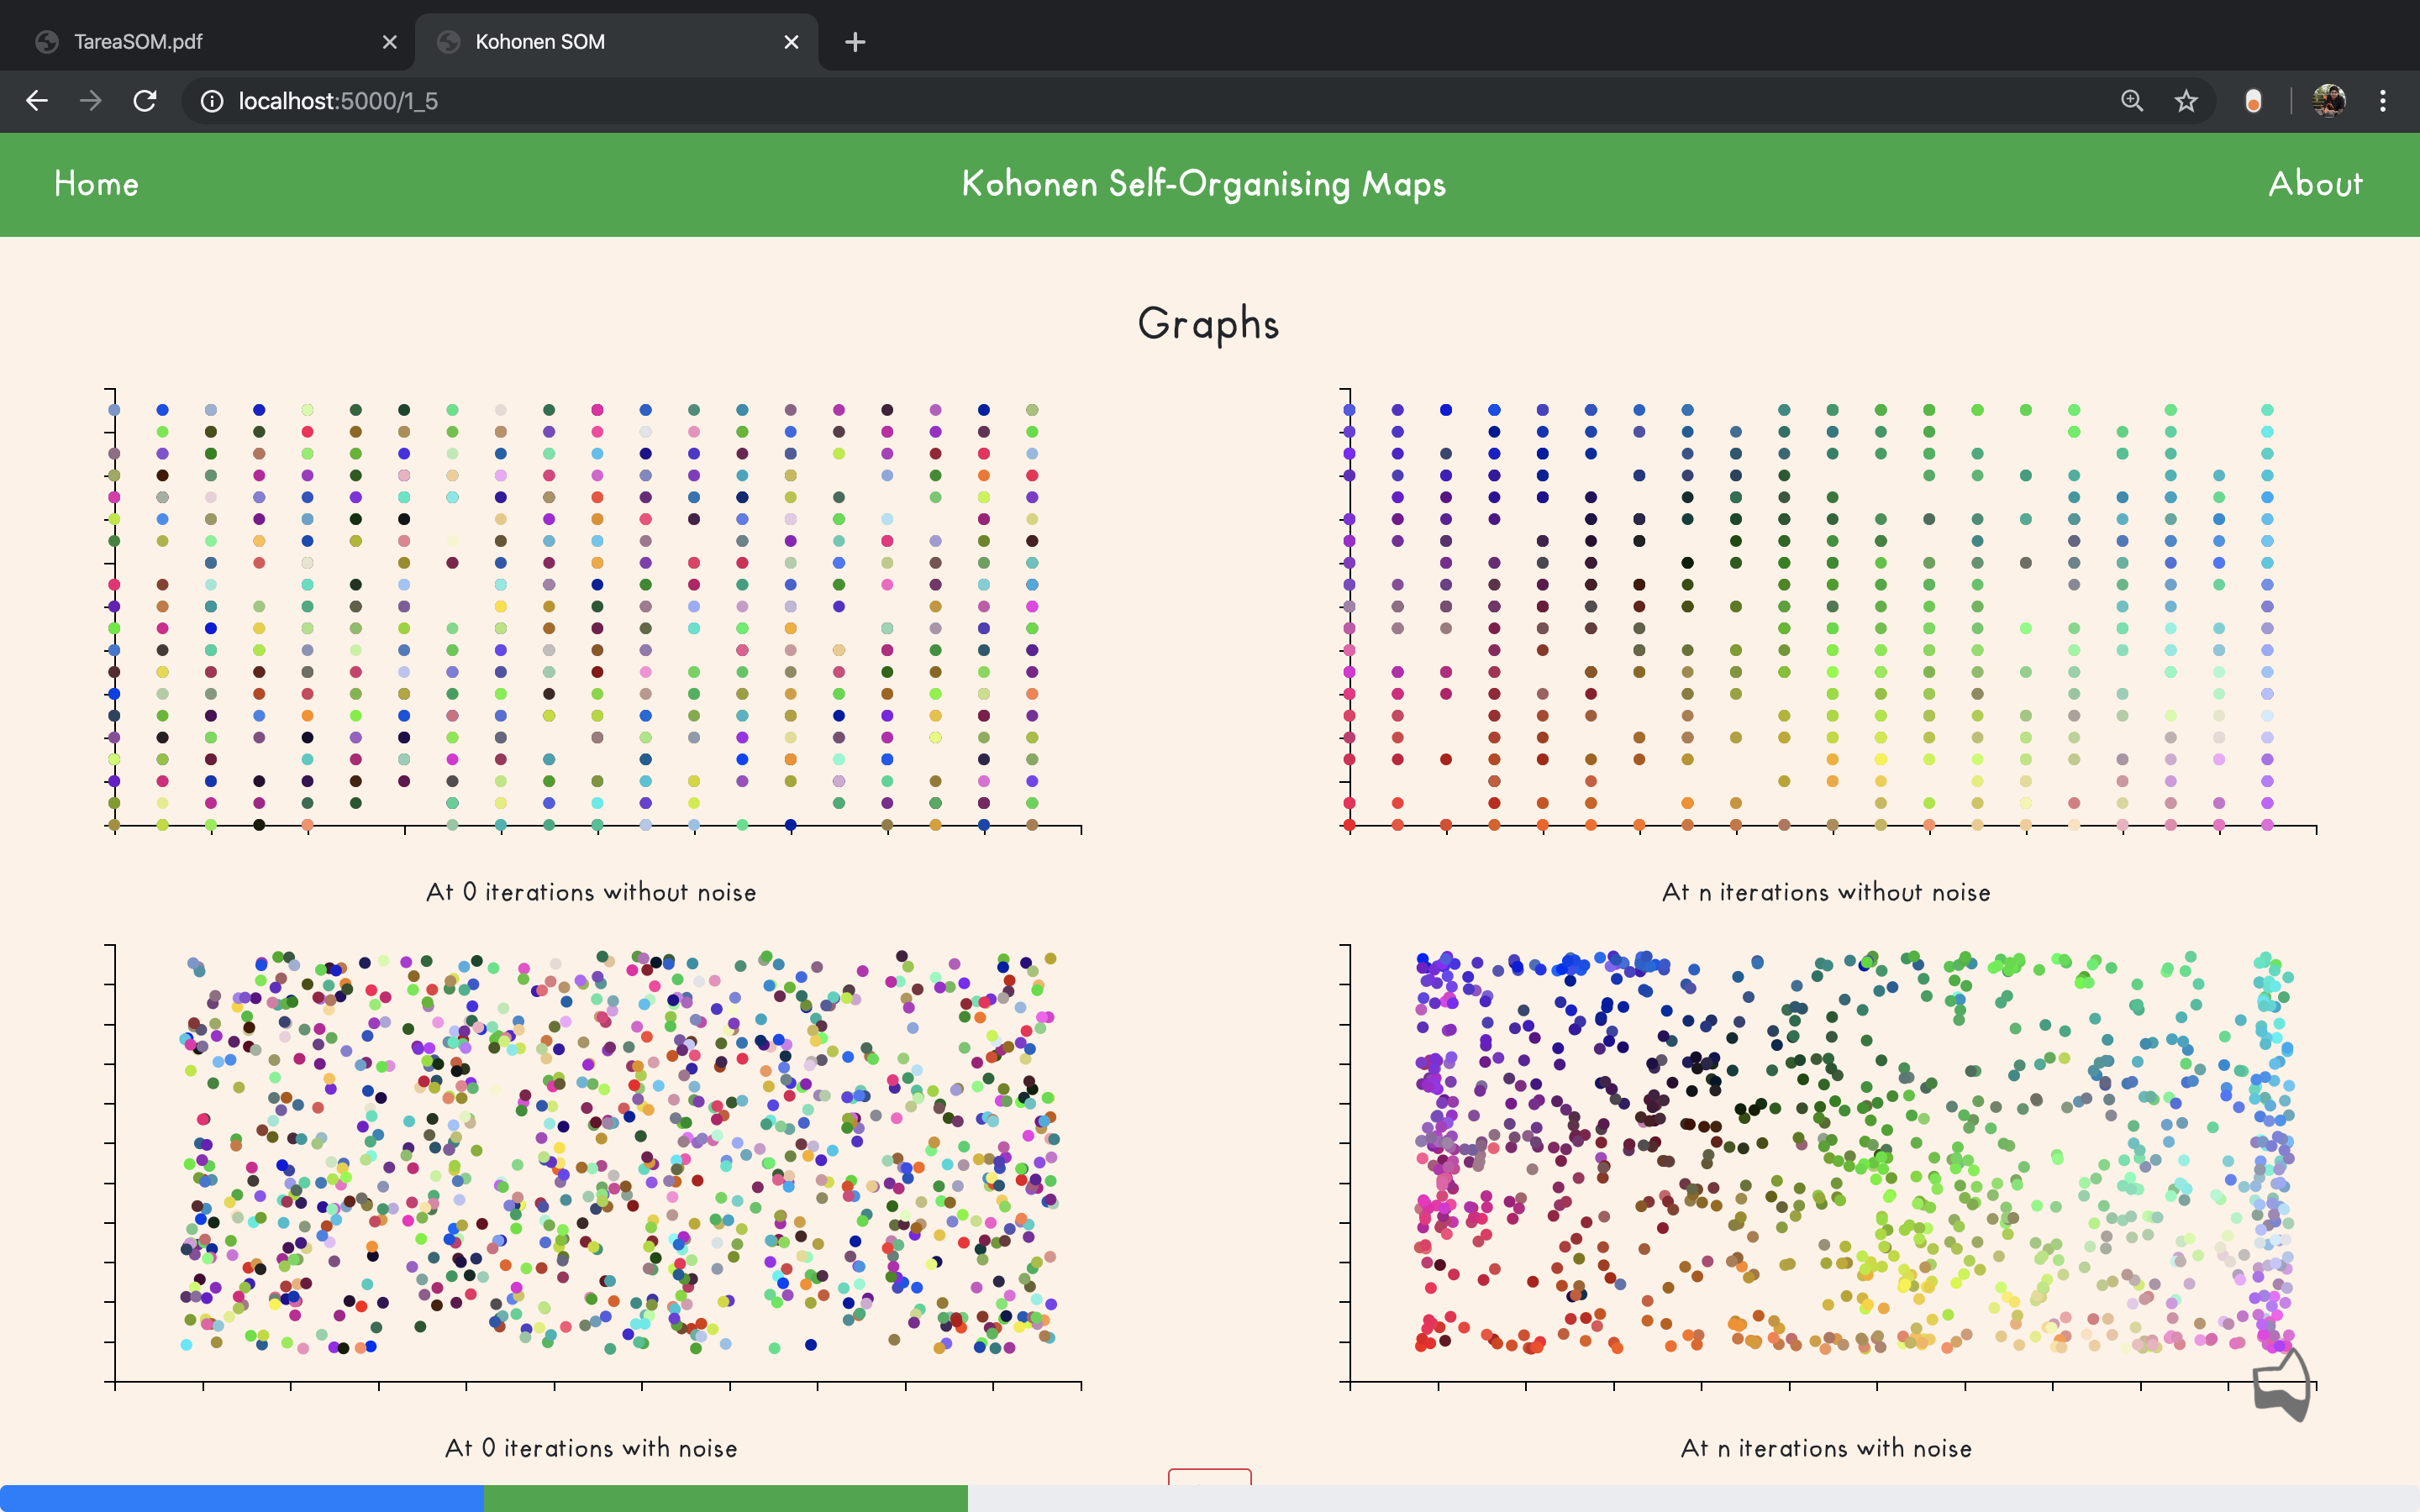
\includegraphics[width=\textwidth]{Tesis8}
      \end{figure}

      \begin{figure}[h!]
        \centering
        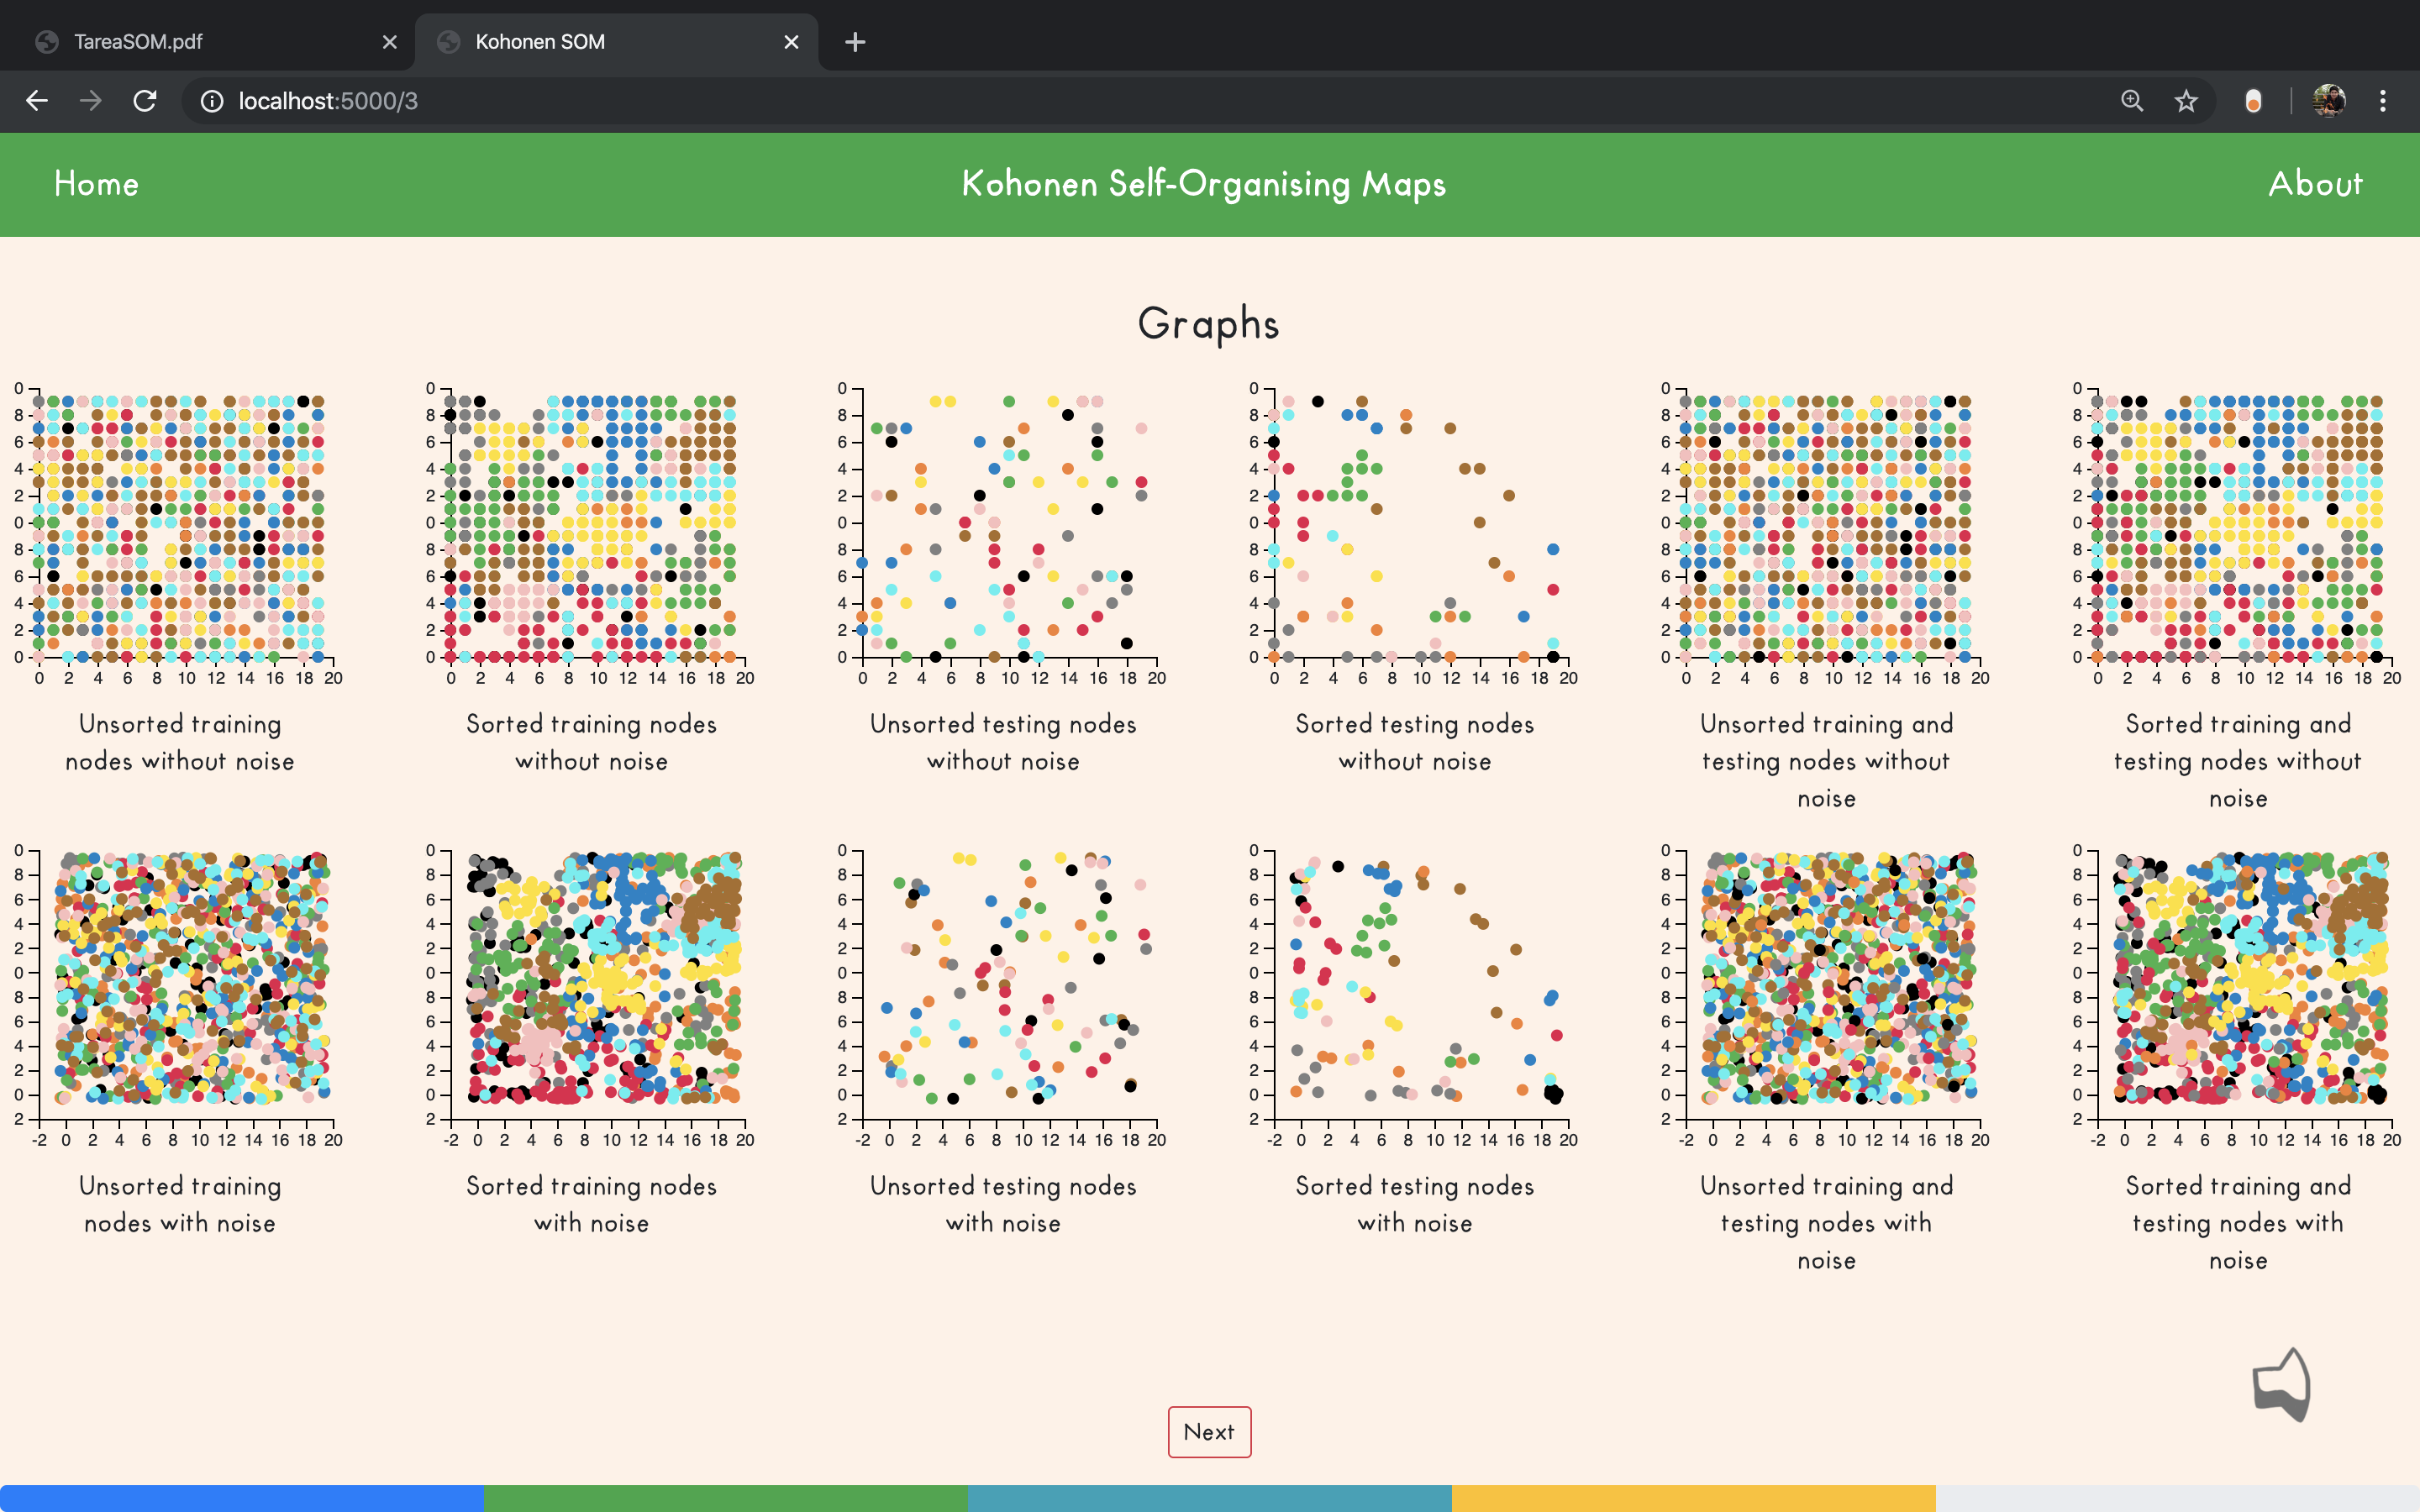
\includegraphics[width=\textwidth]{Tesis9}
      \end{figure}


  \clearpage
  \section{Memes}

  \begin{figure}[h!]
    \centering
    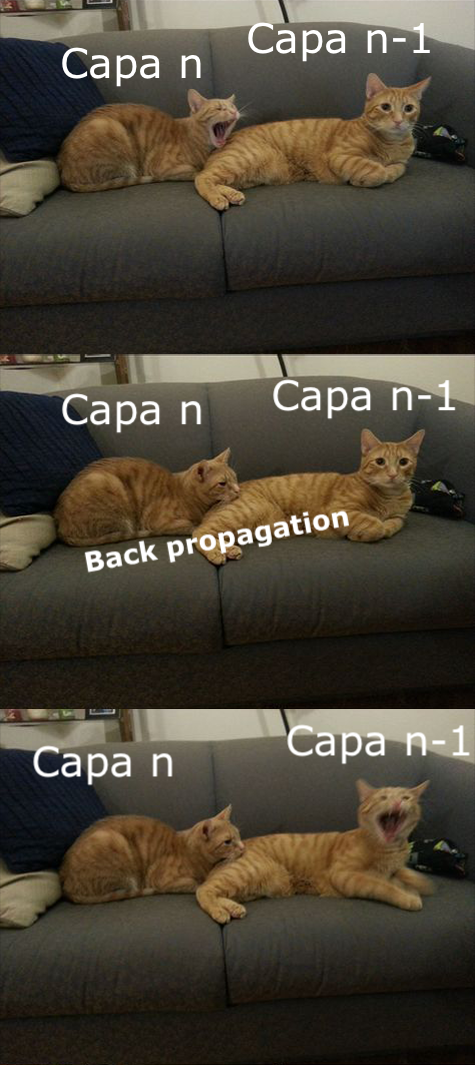
\includegraphics[width=0.3\textwidth]{a}
  \end{figure}


    \begin{thebibliography}{10}

      \bibitem{Visual} 
        Deboeck, G. and Kohonen, T. (1998). 
        Visual explorations in finance with self-organising maps. London: Springer.

        Pueden descargarlo de aquí: (https://www.springer.com/gp/book/9783540762669)


        \bibitem{Dos}

          Guido J Deboeck
          Neural Network World, May 2000
          Financial Applications of Self-Organizing Maps

          Pueden descargarlo de aquí:  (https://pdfs.semanticscholar.org/e46d/77829d20ef37762d16baccc5d91eb114e25e.pdf)

        \bibitem{Tres}
            
        Self-Organizing Map: ScienceDirect
        https://www.sciencedirect.com/topics/engineering/self-organizing-map

        \bibitem{Robot}

        Craig Sayers, May 1991, University of Pennsylvania
        Self Organizing Feature Maps and Their Applications to Robotics

        \bibitem{Otro}

        Kohonen Self-Organizing Maps        
        https://towardsdatascience.com/kohonen-self-organizing-maps-a29040d688da

        \bibitem{Tesis}
        Eklavya Sarkar, University of Liverpool
        Artificial Neural Networks: Kohonen Self-Organising Maps

        Link: https://eklavyafcb.github.io/som.html

    \end{thebibliography}


\end{document}